%definira klasu dokumenta 
\documentclass[12pt]{report} 

%prostor izmedu naredbi \documentclass i \begin{document} se zove uvod. U njemu se nalaze naredbe koje se odnose na cijeli dokument

%osnovni LaTex ne može riješiti sve probleme, pa se koriste različiti paketi koji olakšavaju izradu željenog dokumenta
\usepackage[croatian]{babel} 
\usepackage{amssymb}
\usepackage{amsmath}
\usepackage{txfonts}
\usepackage{mathdots}
\usepackage{titlesec}
\usepackage{array}
\usepackage{lastpage}
\usepackage{etoolbox}
\usepackage{tabularray}
\usepackage{color, colortbl}
\usepackage{adjustbox}
\usepackage{geometry}
\usepackage[classicReIm]{kpfonts}
\usepackage{hyperref}
\usepackage{fancyhdr}
\usepackage{tabularx} % Required for controlling table width
\usepackage{float}
\usepackage[T1]{fontenc}
\usepackage[table]{xcolor}

\usepackage{float}
\usepackage{setspace}
\restylefloat{table}


\patchcmd{\chapter}{\thispagestyle{plain}}{\thispagestyle{fancy}}{}{} %redefiniranje stila stranice u paketu fancyhdr

%oblik naslova poglavlja
\titleformat{\chapter}{\normalfont\huge\bfseries}{\thechapter.}{20pt}{\Huge}
\titlespacing{\chapter}{0pt}{0pt}{40pt}


\linespread{1.3} %razmak između redaka

\geometry{a4paper, left=1in, top=1in,}  %oblik stranice

\hypersetup{ colorlinks, citecolor=black, filecolor=black, linkcolor=black,	urlcolor=black }   %izgled poveznice


%prored smanjen između redaka u nabrajanjima i popisima
\newenvironment{packed_enum}{
	\begin{enumerate}
		\setlength{\itemsep}{0pt}
		\setlength{\parskip}{0pt}
		\setlength{\parsep}{0pt}
	}{\end{enumerate}}

\newenvironment{packed_item}{
	\begin{itemize}
		\setlength{\itemsep}{0pt}
		\setlength{\parskip}{0pt}
		\setlength{\parsep}{0pt}
	}{\end{itemize}}




%boja za privatni i udaljeni kljuc u tablicama
\definecolor{LightBlue}{rgb}{0.9,0.9,1}
\definecolor{LightGreen}{rgb}{0.9,1,0.9}

%Promjena teksta za dugačke tablice
\DefTblrTemplate{contfoot-text}{normal}{Nastavljeno na idućoj stranici}
\SetTblrTemplate{contfoot-text}{normal}
\DefTblrTemplate{conthead-text}{normal}{(Nastavljeno)}
\SetTblrTemplate{conthead-text}{normal}
\DefTblrTemplate{middlehead,lasthead}{normal}{Nastavljeno od prethodne stranice}
\SetTblrTemplate{middlehead,lasthead}{normal}

%podesavanje zaglavlja i podnožja

\pagestyle{fancy}
\lhead{Programsko inženjerstvo}
\rhead{Donori krvi}
\lfoot{Armando Maradona}
\cfoot{stranica \thepage/\pageref{LastPage}}
\rfoot{\today}
\renewcommand{\headrulewidth}{0.2pt}
\renewcommand{\footrulewidth}{0.2pt}


\begin{document} 
	
	
	
	\begin{titlepage}
		\begin{center}
			\vspace*{\stretch{1.0}} %u kombinaciji s ostalim \vspace naredbama definira razmak između redaka teksta
			\LARGE Programsko inženjerstvo\\
			\large Ak. god. 2023./2024.\\
			
			\vspace*{\stretch{3.0}}
			
			\huge Donori krvi\\
			\Large Dokumentacija, Rev. \textit{$1$}\\
			
			\vspace*{\stretch{12.0}}
			\normalsize
			Grupa: \textit Armando Maradona\\
			Voditelj: \textit Zvonko Lelas\\
			
			
			\vspace*{\stretch{1.0}}
			Datum predaje: \textit{$<$dan$>$. $<$mjesec$>$. $<$godina$>$.}\\
	
			\vspace*{\stretch{4.0}}
			
			Nastavnik: \textit Vlado Sruk\\
		
		\end{center}

	
	\end{titlepage}

	
	\tableofcontents


	\chapter{Dnevnik promjena dokumentacije}
		
		\textbf{\textit{Kontinuirano osvježavanje}}\\
				
		
		\begin{longtblr}[
				label=none
			]{
				width = \textwidth, 
				colspec={|X[2]|X[13]|X[3]|X[3]|}, 
				rowhead = 1
			}
			\hline
			\textbf{Rev.}	& \textbf{Opis promjene/dodatka} & \textbf{Autori} & \textbf{Datum}\\[3pt] \hline
			0.1 & Napravljen predložak.	& Bruna Matić & 28.10.2023. 		\\[3pt] \hline 
			0.2	& Dopisane upute za povijest dokumentacije.\newline Dodane reference. & * & 24.08.2013. 	\\[3pt] \hline 
			0.5 & Dodan \textit{Use Case} dijagram i jedan sekvencijski dijagram, funkcionalni i nefunkcionalni zahtjevi i dodatak A & * & 25.08.2013. \\[3pt] \hline 
			0.6 & Arhitektura i dizajn sustava, algoritmi i strukture podataka & * & 26.08.2013. \\[3pt] \hline 
			0.8 & Povijest rada i trenutni status implementacije,\newline Zaključci i plan daljnjeg rada & * & 28.08.2013. \\[3pt] \hline 
			0.9 & Opisi obrazaca uporabe & * & 07.09.2013. \\[3pt] \hline 
			0.10 & Preveden uvod & * & 08.09.2013. \\[3pt] \hline 
			0.11 & Sekvencijski dijagrami & * & 09.09.2013. \\[3pt] \hline 
			0.12.1 & Započeo dijagrame razreda & * & 10.09.2013. \\[3pt] \hline 
			0.12.2 & Nastavak dijagrama razreda & * & 11.09.2013. \\[3pt] \hline 
			\textbf{1.0} & Verzija samo s bitnim dijelovima za 1. ciklus & * & 11.09.2013. \\[3pt] \hline 
			1.1 & Uređivanje teksta -- funkcionalni i nefunkcionalni zahtjevi & * \newline * & 14.09.2013. \\[3pt] \hline 
			1.2 & Manje izmjene:Timer - Brojilo vremena & * & 15.09.2013. \\[3pt] \hline 
			1.3 & Popravljeni dijagrami obrazaca uporabe & * & 15.09.2013. \\[3pt] \hline 
			1.5 & Generalna revizija strukture dokumenta & * & 19.09.2013. \\[3pt] \hline 
			1.5.1 & Manja revizija (dijagram razmještaja) & * & 20.09.2013. \\[3pt] \hline 
			\textbf{2.0} & Konačni tekst predloška dokumentacije  & * & 28.09.2013. \\[3pt] \hline 
			&  &  & \\[3pt] \hline	
		\end{longtblr}
	
	
		\textit{Moraju postojati glavne revizije dokumenata 1.0 i 2.0 na kraju prvog i drugog ciklusa. Između tih revizija mogu postojati manje revizije već prema tome kako se dokument bude nadopunjavao. Očekuje se da nakon svake značajnije promjene (dodatka, izmjene, uklanjanja dijelova teksta i popratnih grafičkih sadržaja) dokumenta se to zabilježi kao revizija. Npr., revizije unutar prvog ciklusa će imati oznake 0.1, 0.2, …, 0.9, 0.10, 0.11.. sve do konačne revizije prvog ciklusa 1.0. U drugom ciklusu se nastavlja s revizijama 1.1, 1.2, itd.}
	\chapter{Opis projektnog zadatka}
		
		Ova web aplikacija omogućuje donatorima krvi da uz što manje muke nađu najbliže lokacije darivanja krvi te im daje mogućnost prisustvovanja u 				raznim akcijama organiziranih od Crvenog Križa ili drugih zavoda. Donor ima pristup svojoj povijesti darivanja što mu omogućava lako izdavanje 					potvrde od prošlih darivanje te datum isteka perioda čekanja ( od svakog darivanja krvi treba proći 4-6 mjeseci ovisno o spolu, radi tetovaža…). 					Svakim darivanjem krvi donor skuplja mogućnost za razne bonuse.
		
		Crvenom Križu i ostalim zavodima ova aplikacija omogućuje lakše organiziranje akcija u slučaju manjka krvi na nekoj lokaciji. Preko aplikacije 					dodjeljuju priznanja, izdavaju potvrde i davaju pozivnice. Također imaju evidenciju o svim darivateljima (ime, prezime, krvna grupa). Zadaća 					administratora je verificiranje podataka te davanje dopuštenja za darivanje.

		Ova aplikacija bi bila u interesu svih ljudi koji su zainteresirani za darivanje krvi, onih koji žele nešto o tome naučiti te onih koji ih organiziraju. Zbog 				lake uporabe lako povezuje donore s mjestima u krizi (bolnicama, organizacijama). Također omogućava povezanost između mjesta darivanja jer im 				daje uvit koliko koje krvi ima koja ustanova.

		Prilikom pokretanja stranice pojavljuje se karta Republike Hrvatske s označenim lokacijama (Zavod za transfuziju KBC Osijek, KBC Rijeka, KBC Split, OB 		Dubrovnik, OB Varaždin, OB Zadar i Hrvatski zavod za transfuzijsku medicinu Zagreb) te prozor s akcijama Crvenog Križa u Hrvatskoj. Klikom na 					lokacije pojavi se prozor u kojem se nalaze akcije za tu lokaciju, postotci zaliha krvi te gumb za prijavu za donaciju. Neregistriranog korisnika stranica 				vodi na registraciju, a korisniku prikazuje registracijski obrazac za donaciju. 
		Neregistrirani korisnik se može prijaviti u aplikaciju kao:

		\begin{packed_item}
			\item donor –  pojavljuju mu se skočni prozorčići s pozivima Crvenog Križa na donacije i akcije, omogućena mu je kontrola osobnih 							podataka, prijava na donacije i akcije, statistika vlastitog doniranja, ispis potvrda i zahtjev za nagradama od Crvenog Križa i drugih zavoda te 					brisanje korisničkog računa
				\begin{packed_item}
					\item potrebne informacije za registraciju
				\end{packed_item}
			\item Crveni Križ – omogućeno mu je objavljivanje akcija, izdavanje potvrda, dodjela priznanja te verificiranje podataka
				\begin{packed_item}
					\item potrebne informacije za registraciju
				\end{packed_item}
			\item zavodi – omogućen uvid u popis donora, brisanje donorskih korisničkih računa i izdavanje akcija
				\begin{packed_item}
					\item potrebne informacije za registraciju
				\end{packed_item}
		\end{packed_item}
		
		Administratori su osobe zaslužne za održavanje aplikacije te se neregistriranom korisniku ne daje pristup prijave kao administrator. 

		Sustav treba podržavati rad više korisnika u stvarnom vremenu.

		Slične web aplikacije:
		\begin{packed_item}
			\item  „GiveBlood“ ( https://www.redcross.org/give-blood.html ):
			Na početnoj web stranici nalaze se obavijesti vezane za različite krvne grupe, krvnu plazmu te različite zanimljivosti vezane uz temu. U alatnoj 					traci nalaze se često pitana pitanja koja su grupirana po temama ( „sve o plazmi“, „zašto dati krv“, „tko može dati krv“,  „proces donacije“). Tu se 			također nalazi tražilica koja traži najbliže lokacije u Engleskoj gdje se može donirati te link s aktualnim zdravstvenim vijestima. Korisnici imaju 					mogućnost prijave i rezervacije termina za donaciju.
			\begin{figure}[H]
				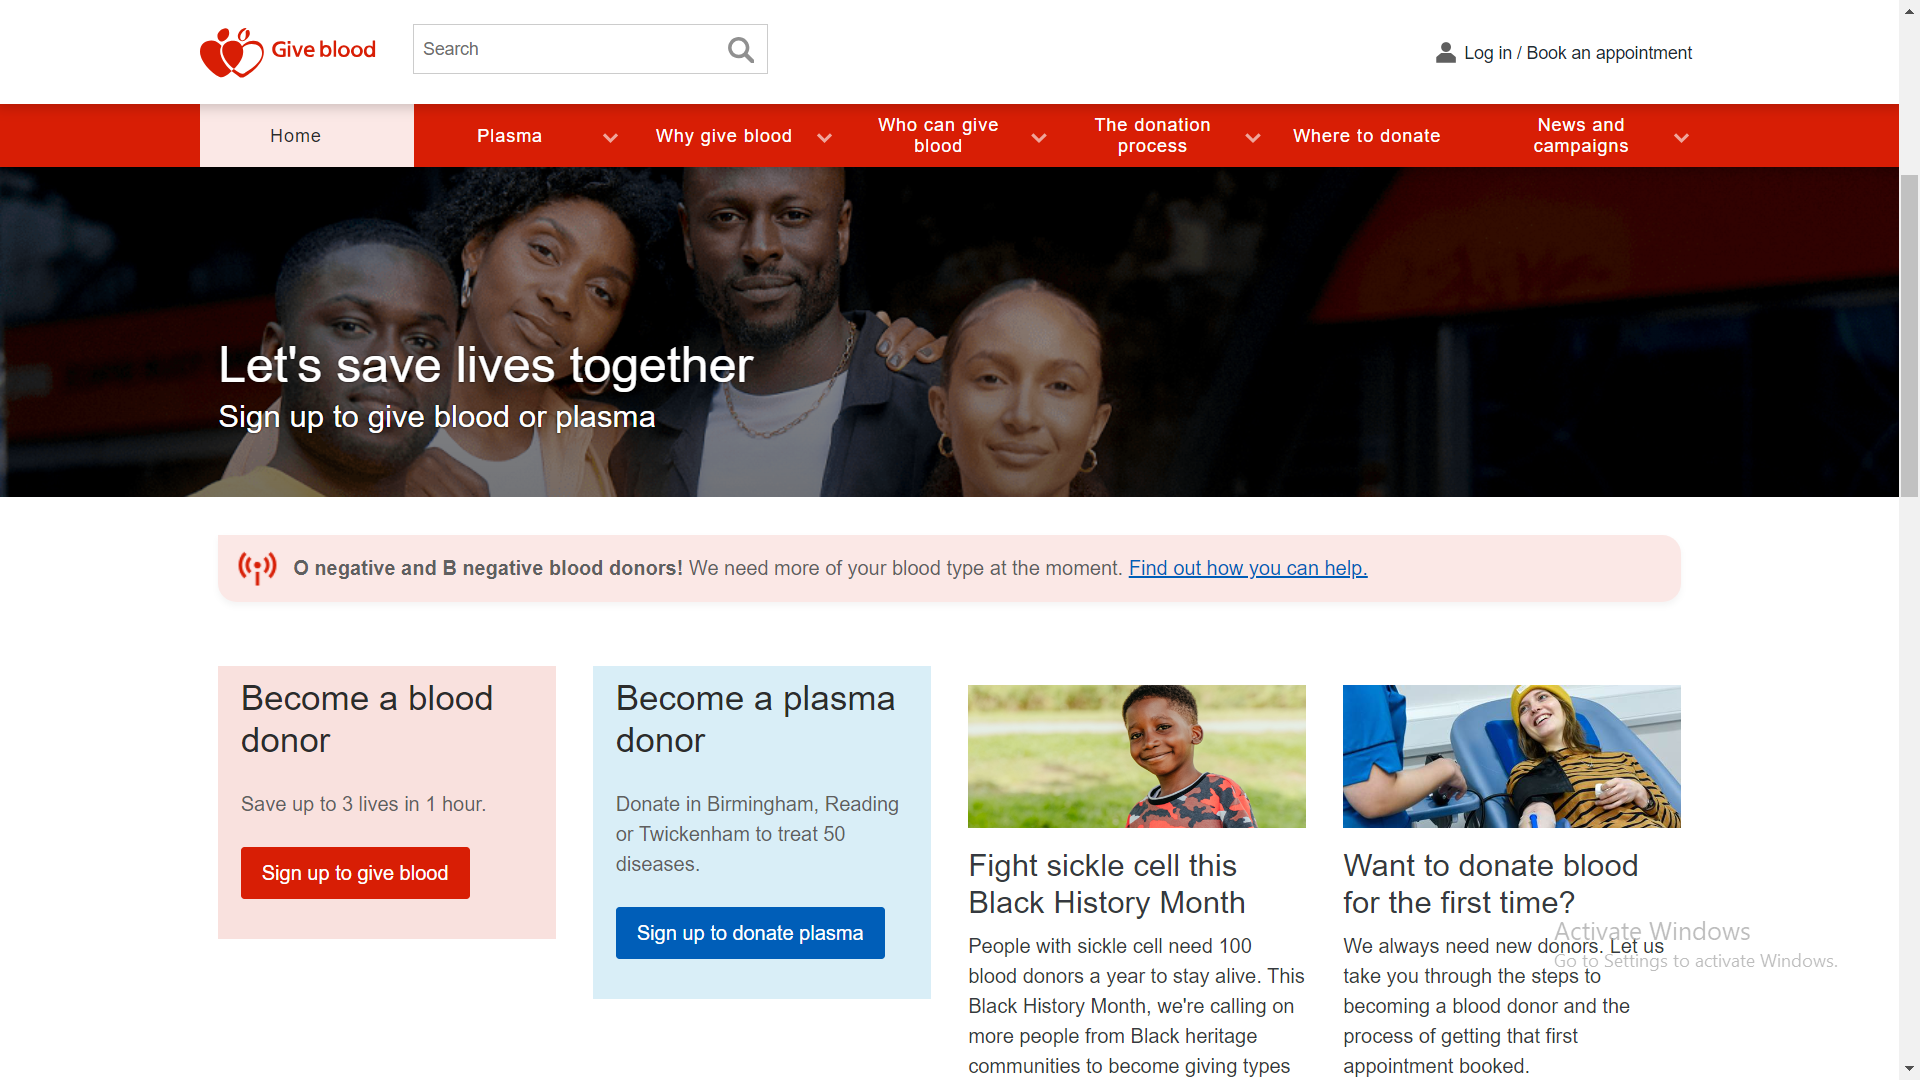
\includegraphics[scale=0.23]{slike/giveblood.PNG} 
				\centering
				\caption{Prikaz glavne stranice GiveBlood-a}
				\label{fig:promjene}
			\end{figure}
			\item „friends2support“ ( https://www.friends2support.org/index.aspx ):
			Web stranica traži davatelje krvi diljem svijeta. Korisnik može unijeti krvnu grupu, državu, županiju, okrug i grad te aplikacija na temelju toga 					traži donatore. Korisnik ima mogućnost registracije. Na stranici se također nalaze razne vijesti, videa i slike o darivanju krvi.
			\begin{figure}[H]
				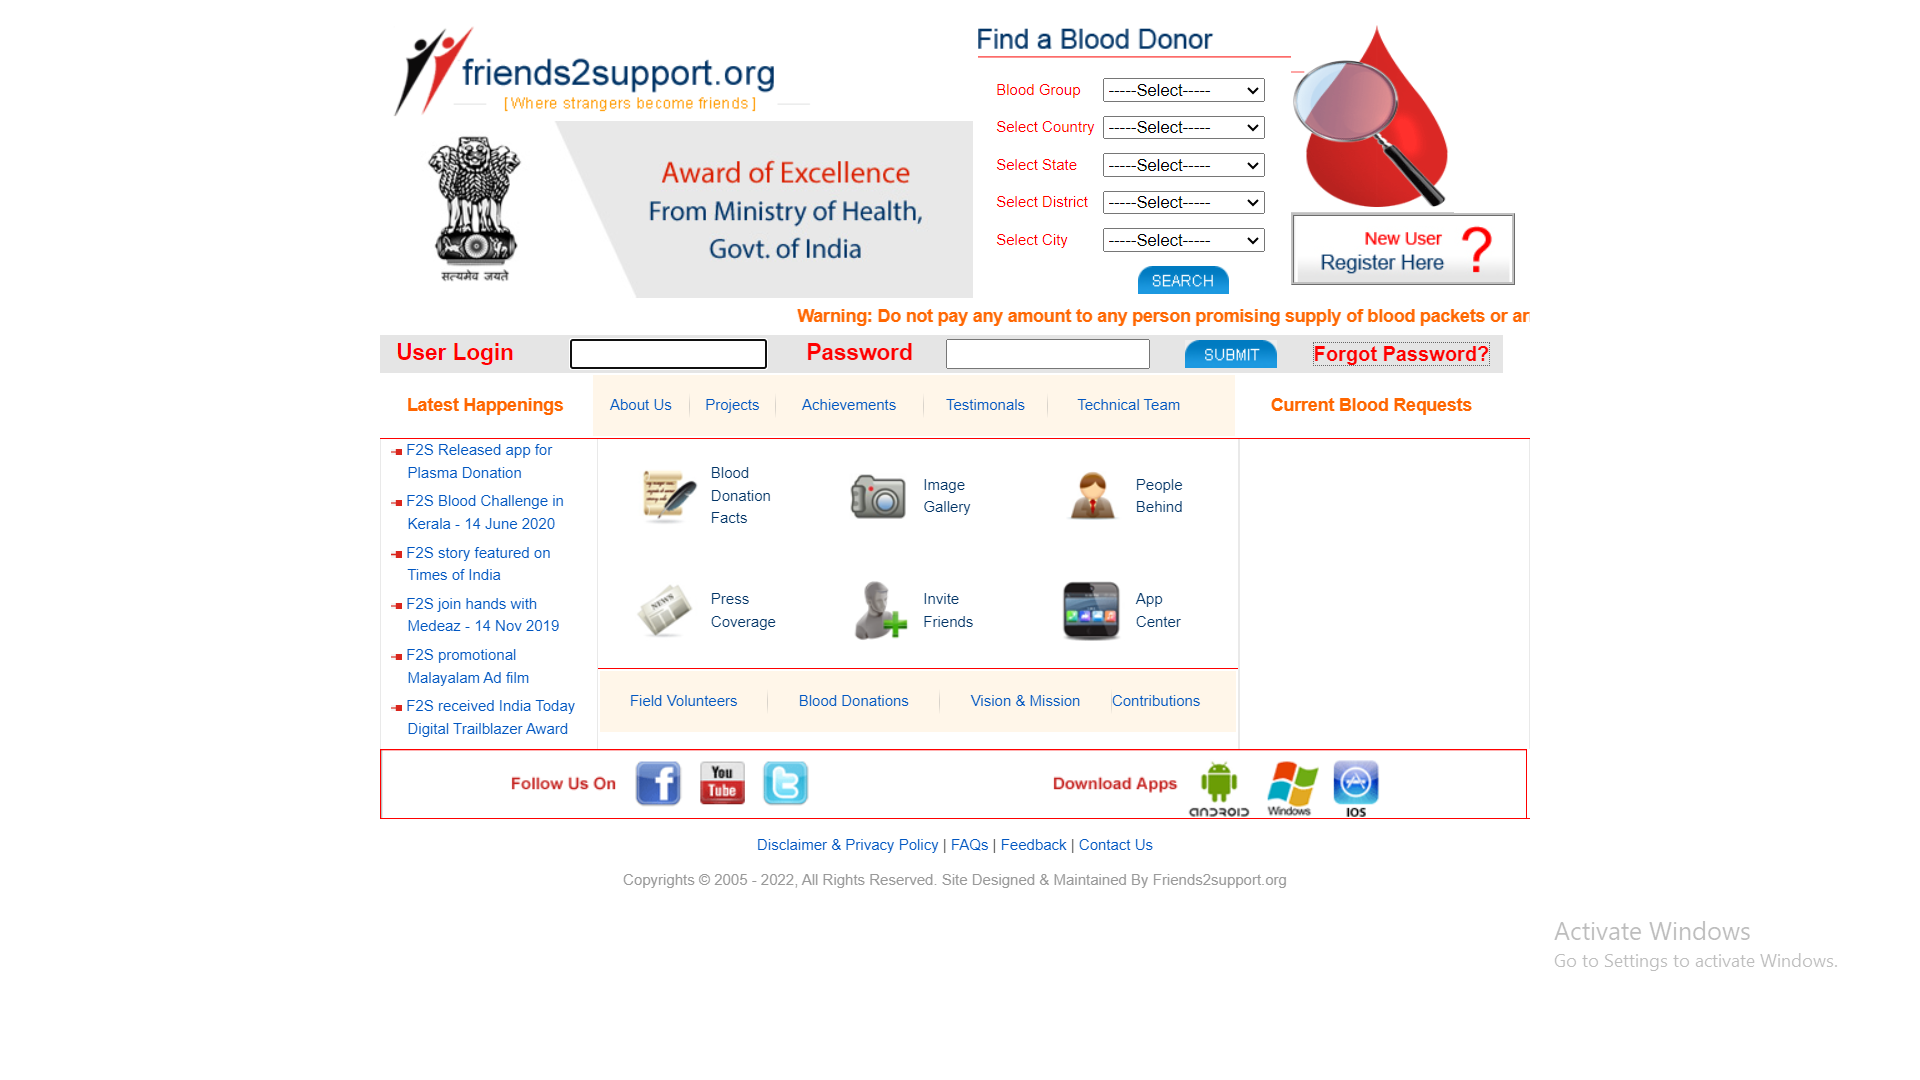
\includegraphics[scale=0.23]{slike/friends2support.PNG} 
				\centering
				\caption{Prikaz glavne stranice friends2support-a}
				\label{fig:promjene}
			\end{figure}
			\item  „vitalant“ ( https://vitalant.org/ ):
			Na početnoj stanici nalaze se elementi preko kojih korisnik  može zakazati termin donacije, naučiti o donaciji te saznati je li poželjni donor. 						Također iskaču aktualne vijesti ili nagradne igre. Na alatnoj traci nalaze se razna pitanja i članci grupirani po temama (o donaciji, o krvi,  o 						poželjnosti, o volonterima i o bolnicama).
			\begin{figure}[H]
				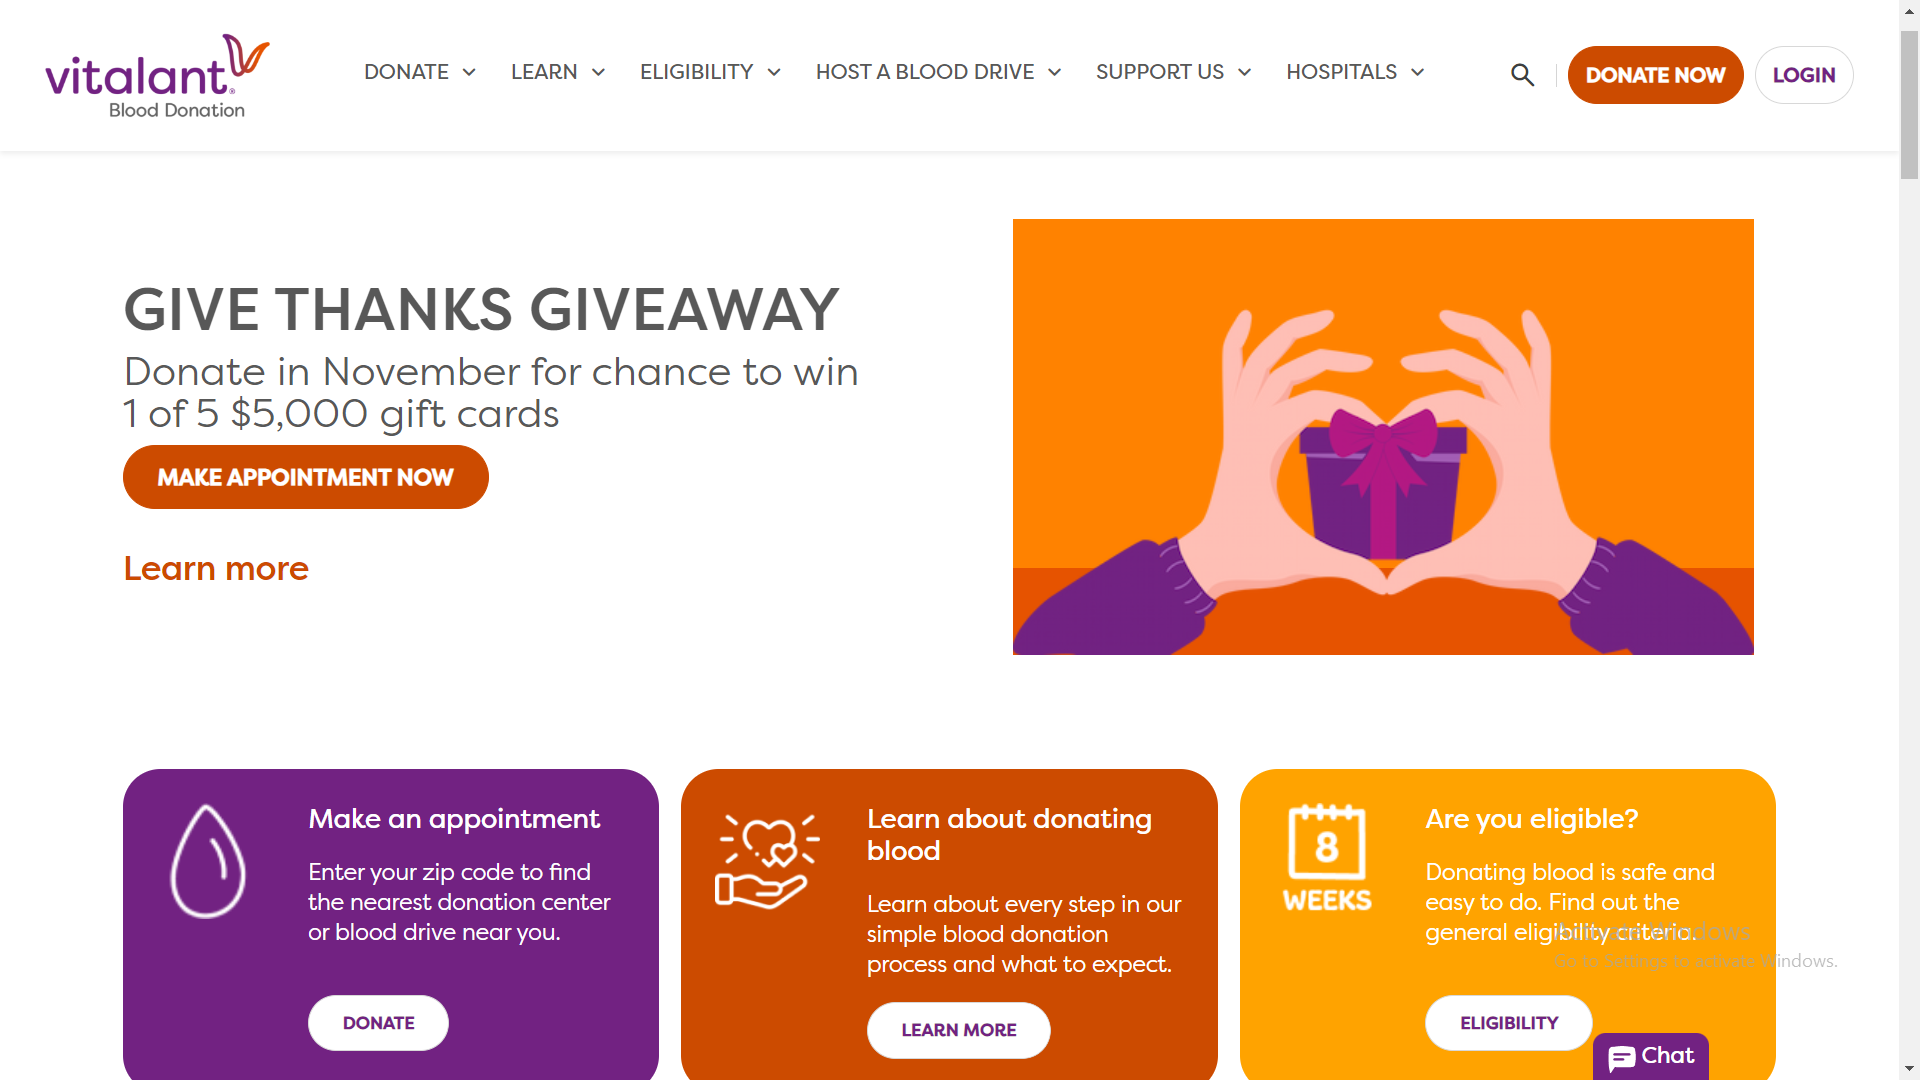
\includegraphics[scale=0.23]{slike/vitalant.PNG} 
				\centering
				\caption{Prikaz glavne stranice vitalant-a}
				\label{fig:promjene}
			\end{figure}
		\end{packed_item}

		\eject
		
		\section{Primjeri u \LaTeX u}
		
		\textit{Ovo potpoglavlje izbrisati.}\\

		U nastavku se nalaze različiti primjeri kako koristiti osnovne funkcionalnosti \LaTeX a koje su potrebne za izradu dokumentacije. Za dodatnu pomoć obratiti se asistentu na projektu ili potražiti upute na sljedećim web sjedištima:
		\begin{itemize}
			\item Upute za izradu diplomskog rada u \LaTeX u - \url{https://www.fer.unizg.hr/_download/repository/LaTeX-upute.pdf}
			\item \LaTeX\ projekt - \url{https://www.latex-project.org/help/}
			\item StackExchange za Tex - \url{https://tex.stackexchange.com/}\\
		
		\end{itemize} 	


		
		\noindent \underbar{podcrtani tekst}, \textbf{podebljani tekst}, 	\textit{nagnuti tekst}\\
		\noindent \normalsize primjer \large primjer \Large primjer \LARGE {primjer} \huge {primjer} \Huge primjer \normalsize
				
		\begin{packed_item}
			
			\item  primjer
			\item  primjer
			\item  primjer
			\item[] \begin{packed_enum}
				\item primjer
				\item[] \begin{packed_enum}
					\item[1.a] primjer
					\item[b] primjer
				\end{packed_enum}
				\item primjer
			\end{packed_enum}
			
		\end{packed_item}
		
		\noindent primjer url-a: \url{https://www.fer.unizg.hr/predmet/proinz/projekt}
		
		\noindent posebni znakovi: \# \$ \% \& \{ \} \_ 
		$|$ $<$ $>$ 
		\^{} 
		\~{} 
		$\backslash$ 
		
		
		\begin{longtblr}[
			label=none,
			entry=none
			]{
				width = \textwidth,
				colspec={|X[8,l]|X[8, l]|X[16, l]|}, 
				rowhead = 1,
			} %definicija širine tablice, širine stupaca, poravnanje i broja redaka naslova tablice
			\hline \SetCell[c=3]{c}{\textbf{naslov unutar tablice}}	 \\ \hline[3pt]
			\SetCell{LightGreen}IDKorisnik & INT	&  	Lorem ipsum dolor sit amet, consectetur adipiscing elit, sed do eiusmod  	\\ \hline
			korisnickoIme	& VARCHAR &   	\\ \hline 
			email & VARCHAR &   \\ \hline 
			ime & VARCHAR	&  		\\ \hline 
			\SetCell{LightBlue} primjer	& VARCHAR &   	\\ \hline 
		\end{longtblr}
		

		\begin{longtblr}[
				caption = {Naslov s referencom izvan tablice},
				entry = {Short Caption},
			]{
				width = \textwidth, 
				colspec = {|X[8,l]|X[8,l]|X[16,l]|}, 
				rowhead = 1,
			}
			\hline
			\SetCell{LightGreen}IDKorisnik & INT	&  	Lorem ipsum dolor sit amet, consectetur adipiscing elit, sed do eiusmod  	\\ \hline
			korisnickoIme	& VARCHAR &   	\\ \hline 
			email & VARCHAR &   \\ \hline 
			ime & VARCHAR	&  		\\ \hline 
			\SetCell{LightBlue} primjer	& VARCHAR &   	\\ \hline 
		\end{longtblr}
	


		
		
		%unos slike
		\begin{figure}[H]
			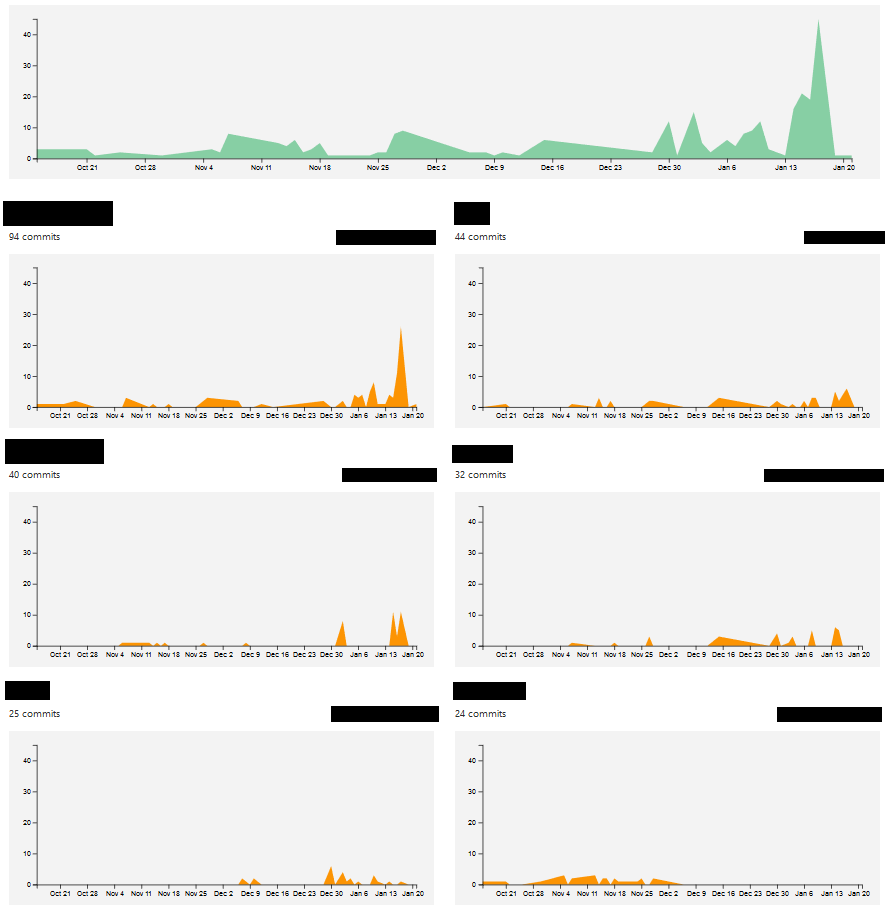
\includegraphics[scale=0.4]{slike/aktivnost.PNG} %veličina slike u odnosu na originalnu datoteku i pozicija slike
			\centering
			\caption{Primjer slike s potpisom}
			\label{fig:promjene}
		\end{figure}
		
		\begin{figure}[H]
			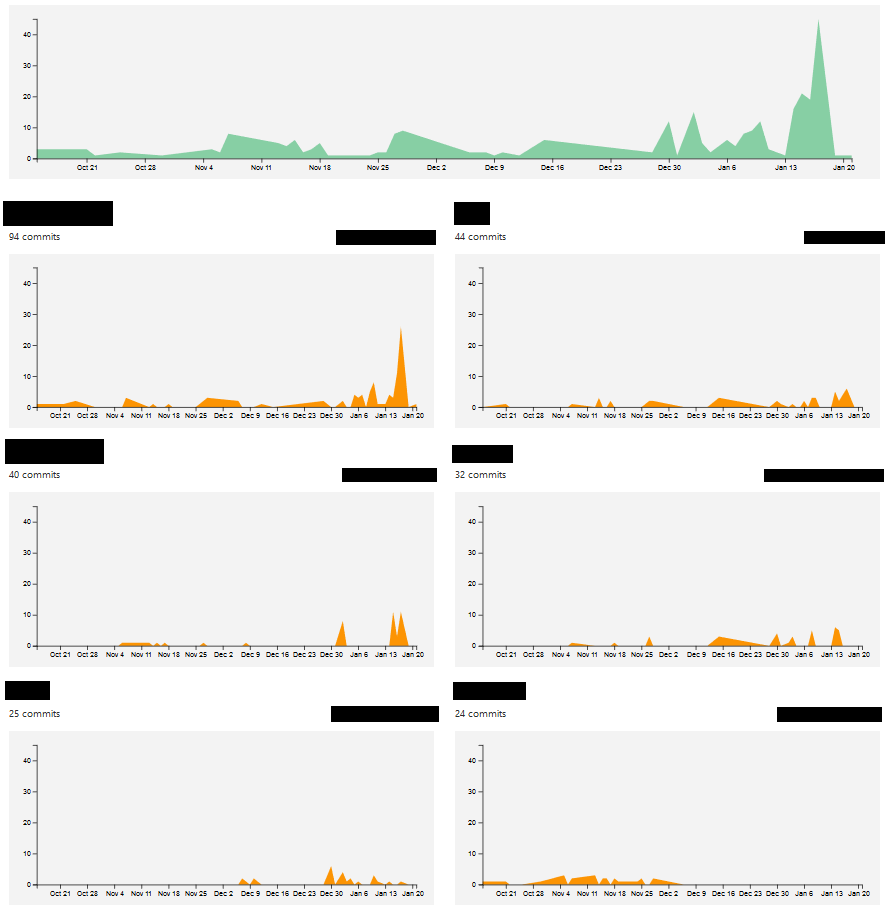
\includegraphics[width=\textwidth]{slike/aktivnost.PNG} %veličina u odnosu na širinu linije
			\caption{Primjer slike s potpisom 2}
			\label{fig:promjene2} %label mora biti drugaciji za svaku sliku
		\end{figure}
		
		Referenciranje slike \ref{fig:promjene2} u tekstu.
		
		\eject
		
	
	\chapter{Specifikacija programske potpore}
		
	\section{Funkcionalni zahtjevi}
			
			\noindent \textbf{Dionici:}
			
			\begin{packed_enum}
				
				\item Donor
				\item Zavod
				\item Crveni Križ
				\item Administrator
				\item Razvojni tim ( Bruna Matić, Bruno Galić, Jana Matić, Jelena Lončar, Nikola Borzić, Nikola Marić, Zvonko Lelas )
				\item Asistent predmeta ( Mateja Golec )
				\item profesor predmeta ( Vlado Sruk )
				
			\end{packed_enum}
			
			\noindent \textbf{Aktori i njihovi funkcionalni zahtjevi:}
			
			
			\begin{packed_enum}
				\item  \underbar{Donor (sudionik) može:}
				
				\begin{packed_enum}
					
					\item pristupiti podacima
					\begin{packed_enum}
						
						\item pristup osobnim podacima (ime, prezime, krvna grupa)
						\item  pristupiti svojoj povijesti darivanja
						\item  pristupiti informacijama o akcijama
						\item pristupiti informacijama o količini krvi u pojedinim gradovima
						\item brisanje svog korisničkog računa
				
					\end{packed_enum}

					\item vidjeti koliki mu je period čekanja do sljedećeg darivanja
					\item prijava na akcije
					\item primanje obavijesti od zavoda u slučaju manjka krvi
					\item potvrđivanje pozivnica za darivanje
					\item pristup lokacijama na karti u kojima su organizirana doniranja krvi
					
				\end{packed_enum}
				\item  \underbar{Neregistrirani korisnik (sudionik) može:}
					\begin{packed_enum}
						
						\item vidjeti kartu lokacija za doniranje
						\item vidjeti akcije u kartici
						\item registrirati se
						\begin{packed_enum}
						
						\item kao donor
						\item  kao Crveni Križ
						\item  kao zavod
				
					\end{packed_enum}
				
					\end{packed_enum}
				\item  \underbar{Crveni Križ (inicijator) može:}
				
				\begin{packed_enum}
					
					\item izdavati akcije
					\item dodjeljivati priznanja (nagrade)
					\item evidencija darivatelja
					\item izdavanje potvrda
					\item davanje pozivnica
				\end{packed_enum}

				\item \underbar{Zavod (inicijator) može:}
				\begin{packed_enum}
					
					\item vidjeti popis donora
					\item brisati korisničke račune
					\item izdavati akcije
				\end{packed_enum}
			
				\item \underbar{Baza podataka (inicijator) može:}
				\begin{packed_enum}
					
					\item pohraniti sve podatke o donorima i njihovim ovlastima
					\item pohranjuje podatke o:
						\begin{packed_enum}
						
							\item lokacijama doniranja
							\item količinama krvi
							\item akcijama
							\item odzivima na akcije
						\end{packed_enum}
				\end{packed_enum}
			
			\end{packed_enum}
			
			\eject 
			
			
				
			\subsection{Obrasci uporabe}
				
				\subsubsection{Opis obrazaca uporabe}
				
					\noindent \underbar{\textbf{UC$<$1$>$ -$<$Registracija$>$}}
					\begin{packed_item}
	
						\item \textbf{Glavni sudionik: }$<$Neregistrirani korisnik$>$
						\item  \textbf{Cilj:} $<$Registracija$>$
						\item  \textbf{Sudionici:} $<$Baza podataka$>$
						\item  \textbf{Preduvjet:} $<$Korisnik nema registriran račun s mailom koji želi koristiti$>$
						\item  \textbf{Opis osnovnog tijeka:}
						
						\item[] \begin{packed_enum}
	
							\item $<$Upiši podatke(email, lozinka, godina rođenja, spol, težina, krvna grupa)$>$
							\item $<$Potvrdi podatke$>$
							\item $<$Podaci se provjeravaju u bazi podataka$>$
							\item $<$Podatci se spremaju u bazu podataka$>$
							\item $<$Korisnik je sada prijavljen na web stranici te ima mogućnosti kao i Donor$>$
						\end{packed_enum}
						
						\item  \textbf{Opis mogućih odstupanja:}
						
						\item[] \begin{packed_item}
	
							\item[3.a] $<$Email se već koristi$>$
							\item[3.b] $<$Osoba je premlada za darivanje krvi$>$
						\end{packed_item}
					\end{packed_item}
					
					% UC2 - Pregled mogućih nagrada za donore
					\noindent \underbar{\textbf{UC$<$2$>$ -$<$Pregled mogućih nagrada za donore$>$}}
					\begin{packed_item}
						
						\item \textbf{Glavni sudionik:} $<$Neregistrirani korisnik, Donor$>$
						\item \textbf{Cilj:} $<$Pregled nagrada koje možeš dobiti kao donor$>$
						\item \textbf{Sudionici:} $<$Baza podataka$>$
						\item \textbf{Opis osnovnog tijeka:}
						
						\begin{packed_enum}
							
							\item Korisnik odabire opciju za pregled mogućih nagrada
							\item Iz baze podataka povlače se ažurni podaci o nagradama koje donor može ostvariti
							\item Korisniku se prikazuju podaci
							
						\end{packed_enum}
						
					\end{packed_item}
					
					% UC3 - Pregled uvjeta za darivanje krvi
					\noindent \underbar{\textbf{UC$<$3$>$ -$<$Pregled uvjeta za darivanje krvi$>$}}
					\begin{packed_item}
						
						\item \textbf{Glavni sudionik:} $<$Neregistrirani korisnik, Donor$>$
						\item \textbf{Cilj:} $<$Pregled uvjeta koje moraš ispuniti da bi darivao krv$>$
						\item \textbf{Sudionici:} $<$Baza podataka$>$
						\item \textbf{Opis osnovnog tijeka:}
						
						\begin{packed_enum}
							
							\item Korisnik odabire opciju za pregled uvjeta
							\item Iz baze podataka povlače se ažurni podaci o uvjetima za darivanje krvi
							\item Korisniku se prikazuju podaci
							
						\end{packed_enum}
						
					\end{packed_item}
					
					% UC4 - Pregled statusa zaliha krvi
					\noindent \underbar{\textbf{UC$<$4$>$ -$<$Pregled statusa zaliha krvi$>$}}
					\begin{packed_item}
						
						\item \textbf{Glavni sudionik:} $<$Donor, Neregistrirani korisnik$>$
						\item \textbf{Cilj:} $<$Pregled količine krvi po krvnim grupama u zavodima$>$
						\item \textbf{Sudionici:} $<$Baza podataka$>$
						\item \textbf{Opis osnovnog tijeka:}
						
						\begin{packed_enum}
							
							\item Korisnik odabire zavod za koji želi vidjeti stanje
							\item Povlačimo aktualne podatke iz baze podataka
							\item Prikaz podataka
							
						\end{packed_enum}
						
					\end{packed_item}
					
					% UC5 - Pregled obavijesti o akcijama
					\noindent \underbar{\textbf{UC$<$5$>$ -$<$Pregled obavijesti o akcijama$>$}}
					\begin{packed_item}
						
						\item \textbf{Glavni sudionik:} $<$Donor, Neregistrirani korisnici$>$
						\item \textbf{Cilj:} $<$Pregled obavijesti$>$
						\item \textbf{Sudionici:} $<$Baza podataka$>$
						\item \textbf{Opis osnovnog tijeka:}
						
						\begin{packed_enum}
							
							\item Korisnik odabire stranicu za pregled obavijesti
							\item Povlačimo aktualne podatke iz baze podataka
							\item Korisnik može čitati podatke
							
						\end{packed_enum}
						
					\end{packed_item}
					
					% UC6 - Pregled karte RH s označenim lokacijama
					\noindent \underbar{\textbf{UC$<$6$>$ -$<$Pregled karte RH s označenim lokacijama$>$}}
					\begin{packed_item}
						
						\item \textbf{Glavni sudionik:} $<$Neregistrirani korisnik, Donor$>$
						\item \textbf{Cilj:} $<$Prikaz lokacija zavoda$>$
						\item \textbf{Sudionici:} $<$Baza podataka$>$
						\item \textbf{Opis osnovnog tijeka:}
						
						\begin{packed_enum}
							
							\item Korisnik odabire kartu
							\item Na karti Republike Hrvatske nalaze se lokacije gdje se može darivati krv
							\item Korisnik ima opciju odabrati pojedinu lokaciju te vidjeti stanje zavoda (UC$<$4$>$)
							
						\end{packed_enum}
						
					\end{packed_item}
					
					% UC7 - Prijava
					\noindent \underbar{\textbf{UC$<$7$>$ -$<$Prijava$>$}}
					\begin{packed_item}
						
						\item \textbf{Glavni sudionik:} $<$Donor$>$
						\item \textbf{Cilj:} $<$Prijava$>$
						\item \textbf{Sudionici:} $<$Baza podataka$>$
						\item \textbf{Preduvjet:} $<$Korisnik ima račun$>$
						\item \textbf{Opis osnovnog tijeka:}
						
						\begin{packed_enum}
							
							\item Unos emaila i lozinke
							\item Provjera u bazi podataka
							\item Korisnik je prebačen u način rada za Donora te je prijavljen
							
						\end{packed_enum}
						
						\item \textbf{Opis mogućih odstupanja:}
						
						\begin{packed_item}
							
							\item[3.a] Račun ne postoji
							\begin{enumerate}
								\item Prebacuje se na Registraciju
							\end{enumerate}
							\item[3.b] Kriva lozinka
							\begin{enumerate}
								\item Ponovi unos lozinke
							\end{enumerate}
							
						\end{packed_item}
						
					\end{packed_item}
					
					% UC8 - Odjava
					\noindent \underbar{\textbf{UC$<$8$>$ -$<$Odjava$>$}}
					\begin{packed_item}
						
						\item \textbf{Glavni sudionik:} $<$Donor$>$
						\item \textbf{Cilj:} $<$Odjava$>$
						\item \textbf{Preduvjet:} $<$Korisnik je prijavljen na web stranici$>$
						\item \textbf{Opis osnovnog tijeka:}
						
						\begin{packed_enum}
							
							\item Korisnik odabire opciju Odjavi se
							\item Korisnik biva odjavljen te ga se prebacuje u način rada za neregistriranog korisnika
							
						\end{packed_enum}
						
					\end{packed_item}
					
					% UC9 – Ažuriranje i pregled osobnih podataka
					\noindent \underbar{\textbf{UC$<$9$>$ -$<$Ažuriranje i pregled osobnih podataka$>$}}
					\begin{packed_item}
						
						\item \textbf{Glavni sudionik:} $<$Donor$>$
						\item \textbf{Cilj:} $<$Pregled i promjena osobnih podataka$>$
						\item \textbf{Sudionici:} $<$Baza podataka$>$
						\item \textbf{Preduvjet:} $<$Korisnik ima račun$>$
						\item \textbf{Opis osnovnog tijeka:}
						
						\begin{packed_enum}
							
							\item Korisnik odabire opciju Moj račun
							\item Iz baze podataka prikazujemo njegove podatke
							\item Korisnik može pregledavati svoje podatke
							\item Korisnik ima opciju uređivanja svojih podataka
							\item Nakon uređivanja potvrđuje promjene
							
						\end{packed_enum}
						
						\item \textbf{Opis mogućih odstupanja:}
						
						\begin{packed_item}
							
							\item[5.a] Nedozvoljene promjene (korisnik nije punoljetan)
							\begin{enumerate}
								\item Javlja se greška te se pita korisnika je li to njegov stvarni datum rođenja
								\item Ako nije, odbacuju se promjene
								\item Ako je, račun se briše te se obavještava korisnika
								
							\end{enumerate}
							
						\end{packed_item}
						
					\end{packed_item}
					
					% UC10 – Pregled povijesti darivanja
					\noindent \underbar{\textbf{UC$<$10$>$ -$<$Pregled povijesti darivanja$>$}}
					\begin{packed_item}
						
						\item \textbf{Glavni sudionik:} $<$Donor$>$
						\item \textbf{Cilj:} $<$Pregled povijesti darivanja$>$
						\item \textbf{Sudionici:} $<$Baza podataka$>$
						\item \textbf{Opis osnovnog tijeka:}
						
						\begin{packed_enum}
							
							\item Korisnik odabire opciju Povijest darivanja
							\item Prikazuju se ažurni podaci iz baze podataka o svim darivanjima krvi
							\item Korisnik ima opciju izdavanja potvrde za pojedinu donaciju (UC$<$12$>$)
							
						\end{packed_enum}
						
					\end{packed_item}
					
					% UC11 – Prijavljivanje za darivanje krvi
					\noindent \underbar{\textbf{UC$<$11$>$ -$<$Prijavljivanje za darivanje krvi$>$}}
					\begin{packed_item}
						
						\item \textbf{Glavni sudionik:} $<$Donor$>$
						\item \textbf{Cilj:} $<$Rezervacija termina za doniranje krvi$>$
						\item \textbf{Sudionici:} $<$Baza podataka, Zavod$>$
						\item \textbf{Preduvjet:} $<$Prošlo je dovoljno vremena od zadnje donacije, korisnik nije prijavio ništa izvanredno (bolest, tetovaže…)$>$
						\item \textbf{Opis osnovnog tijeka:}
						
						\begin{packed_enum}
							
							\item Korisnik odabire opciju Rezervacija (za određeni zavod)
							\item Iz baze podataka prikazujemo podatke (slobodni termini)
							\item Korisnik odabire slobodni termin
							\item Korisnik potvrđuje dolazak na odabrani termin
							\item Termin se sprema u bazu podataka te se obavještava zavod
							
						\end{packed_enum}
						
						\item \textbf{Opis mogućih odstupanja:}
						
						\begin{packed_item}
							
							\item[4.a] U međuvremenu, za vrijeme rezerviranja, termin je popunjen
							\begin{enumerate}
								\item Obavještava se korisnika o neuspjehu rezervacije te se ponovno nudi mogućnost rezervacije
							\end{enumerate}
							
						\end{packed_item}
						
					\end{packed_item}
					
					% UC12 – Ispis potvrda i zahtjev za nagradama
					\noindent \underbar{\textbf{UC$<$12$>$ -$<$Ispis potvrda i zahtjev za nagradama$>$}}
					\begin{packed_item}
						
						\item \textbf{Glavni sudionik:} $<$Donor$>$
						\item \textbf{Cilj:} $<$Izdavanje potvrda o darivanju, bonusa i ispričnica$>$
						\item \textbf{Sudionici:} $<$Baza podataka$>$
						\item \textbf{Opis osnovnog tijeka:}
						
						\begin{packed_enum}
							
							\item Korisnik odabire opciju Dokumenti
							\item Prikazuju se termini na kojima je potvrđen dolazak Donora
							\item Korisnik odabire termin te ima opciju preuzimanja Potvrde o darivanju ili Ispričnice
							\item Ako je korisnik ostvario bonuse, također ima opciju preuzeti iste
							
						\end{packed_enum}
						
					\end{packed_item}
					
					% UC13 – Brisanje korisničkog računa
					\noindent \underbar{\textbf{UC$<$13$>$ -$<$Brisanje korisničkog računa$>$}}
					\begin{packed_item}
						
						\item \textbf{Glavni sudionik:} $<$Donor$>$
						\item \textbf{Cilj:} $<$Brisanje korisničkog računa$>$
						\item \textbf{Sudionici:} $<$Baza podataka$>$
						\item \textbf{Opis osnovnog tijeka:}
						
						\begin{packed_enum}
							
							\item Korisnik odabire opciju Obriši račun
							\item Korisnika se pita je li siguran da želi obrisati račun
							\item Korisnik potvrđuje te račun biva obrisan iz baze podataka zajedno sa svim podacima o računu
							\item Korisnik biva prebačen u način rada za Neregistriranog korisnika
							
						\end{packed_enum}
						
					\end{packed_item}
					
					% UC14 – Prijavljivanje za obavještavanje
					\noindent \underbar{\textbf{UC$<$14$>$ -$<$Prijavljivanje za obavještavanje$>$}}
					\begin{packed_item}
						
						\item \textbf{Glavni sudionik:} $<$Donor$>$
						\item \textbf{Cilj:} $<$Subscription na email listu$>$
						\item \textbf{Sudionici:} $<$Baza podataka$>$
						\item \textbf{Opis osnovnog tijeka:}
						
						\begin{packed_enum}
							
							\item Korisnik odabire da želi primati obavijesti
							\item Korisnik se stavlja na email listu
							\item Svaka obavijest koja dolazi na web stranicu također se šalje svima sa email liste
							\item Korisnik također ima opciju odjave s email liste
							
						\end{packed_enum}
						
					\end{packed_item}
					
					% UC15 – Registracija kao CK/Zavod
					\noindent \underbar{\textbf{UC$<$15$>$ -$<$Registracija kao CK/Zavod$>$}}
					\begin{packed_item}
						
						\item \textbf{Glavni sudionik:} $<$Zavod, Crveni Križ$>$
						\item \textbf{Cilj:} $<$Registracija$>$
						\item \textbf{Sudionici:} $<$Baza podataka, Zavod, Crveni Križ$>$
						\item \textbf{Opis osnovnog tijeka:}
						
						\begin{packed_enum}
							
							\item Korisnik odabire opciju registracije kao Zavod/CK
							\item Korisnik unosi podatke te čeka potvrdu
							\item U slučaju da se registrira kao Zavod, može ga potvrditi samo taj Zavod za koji se registrira ili Crveni Križ
							\item U slučaju da se registrira kao Crveni Križ, može ga potvrditi samo Crveni Križ
							\item Kada biva potvrđen, dobiva obavijest na email
							
						\end{packed_enum}
						
					\end{packed_item}
					
					% UC16 – Uvid u popis donora
					\noindent \underbar{\textbf{UC$<$16$>$ -$<$Uvid u popis donora$>$}}
					\begin{packed_item}
						
						\item \textbf{Glavni sudionik:} $<$Zavod, Crveni Križ$>$
						\item \textbf{Cilj:} $<$Pregled donora$>$
						\item \textbf{Sudionici:} $<$Baza podataka$>$
						\item \textbf{Opis osnovnog tijeka:}
						
						\begin{packed_enum}
							
							\item Korisnik odabire opciju Pregled donora
							\item Korisnik dobiva popis svih donora te pregled njihovih podataka (ne baš svih)
							
						\end{packed_enum}
						
					\end{packed_item}
					
					% UC17 – Objava akcija darivanja krvi
					\noindent \underbar{\textbf{UC$<$17$>$ -$<$Objava akcija darivanja krvi$>$}}
					\begin{packed_item}
						
						\item \textbf{Glavni sudionik:} $<$Zavod, Crveni Križ$>$
						\item \textbf{Cilj:} $<$Objava akcija$>$
						\item \textbf{Sudionici:} $<$Donor, Neregistrirani korisnik$>$
						\item \textbf{Opis osnovnog tijeka:}
						
						\begin{packed_enum}
							
							\item Korisnik ima opciju objaviti akciju (postaviti objavu) koju će vidjeti svi Korisnici (Donori i Neregistrirani korisnici)
							\item Objava se također šalje svima prijavljenima na email listu
							
						\end{packed_enum}
						
					\end{packed_item}
					
					% UC18 – Komunikacija s Donorima
					\noindent \underbar{\textbf{UC$<$18$>$ -$<$Komunikacija s Donorima$>$}}
					\begin{packed_item}
						
						\item \textbf{Glavni sudionik:} $<$Crveni Križ, Zavod$>$
						\item \textbf{Cilj:} $<$Komunikacija s Donorima$>$
						\item \textbf{Sudionici:} $<$Donor$>$
						\item \textbf{Opis osnovnog tijeka:}
						
						\begin{packed_enum}
							
							\item Korisnik šalje hitnu obavijest svima ili određenim krvnim grupama zbog nestašice krvi
							
						\end{packed_enum}
						
					\end{packed_item}
					
					% UC19 – Pregled statistike o donacijama
					\noindent \underbar{\textbf{UC$<$19$>$ -$<$Pregled statistike o donacijama$>$}}
					\begin{packed_item}
						
						\item \textbf{Glavni sudionik:} $<$Zavod, Crveni Križ$>$
						\item \textbf{Cilj:} $<$Pregled statistike$>$
						\item \textbf{Sudionici:} $<$Baza podataka$>$
						\item \textbf{Opis osnovnog tijeka:}
						
						\begin{packed_enum}
							
							\item Korisnik odabire opciju Statistika
							\item Računa se ažurna statistika iz baze podataka
							\item Zavodima se prikazuje statistika samo za njihov zavod
							\item Crveni Križ vidi statistiku svih zavoda
							
						\end{packed_enum}
						
					\end{packed_item}
					
					% UC20 – Izdavanje potvrda
					\noindent \underbar{\textbf{UC$<$20$>$ -$<$Izdavanje potvrda$>$}}
					\begin{packed_item}
						
						\item \textbf{Glavni sudionik:} $<$Crveni Križ$>$
						\item \textbf{Cilj:} $<$Izdavanje potvrda o darivanju, bonusa i ispričnica$>$
						\item \textbf{Sudionici:} $<$Baza podataka$>$
						\item \textbf{Opis osnovnog tijeka:}
						
						\begin{packed_enum}
							
							\item Korisnik može potvrditi zahtjev za potvrdu
							
						\end{packed_enum}
						
					\end{packed_item}
					
					% UC21 – Verifikacija podataka
					\noindent \underbar{\textbf{UC$<$21$>$ -$<$Verifikacija podataka$>$}}
					\begin{packed_item}
						
						\item \textbf{Glavni sudionik:} $<$Crveni Križ$>$
						\item \textbf{Cilj:} $<$Verifikacija podataka$>$
						\item \textbf{Sudionici:} $<$Baza podataka$>$
						\item \textbf{Opis osnovnog tijeka:}
						
						\begin{packed_enum}
							
							\item Korisnik može verificirati podatke Donora
							\item Korisnik može potvrditi i odbiti registraciju za Zavod/Crveni Križ
							
						\end{packed_enum}
						
					\end{packed_item}
					
					% UC22 – Brisanje donorskih korisničkih računa
					\noindent \underbar{\textbf{UC$<$22$>$ -$<$Brisanje donorskih korisničkih računa$>$}}
					\begin{packed_item}
						
						\item \textbf{Glavni sudionik:} $<$Crveni Križ$>$
						\item \textbf{Cilj:} $<$Brisanje računa$>$
						\item \textbf{Sudionici:} $<$Baza podataka, Donor$>$
						\item \textbf{Opis osnovnog tijeka:}
						
						\begin{packed_enum}
							
							\item Korisnik odabire opciju Brisanja korisničkog računa
							\item Korisnik mora napisati razlog brisanja korisničkog računa
							\item Korisnički račun se briše iz baze podataka, te se pohranjuje da je račun obrisan i razlog brisanja
							
						\end{packed_enum}
						
					\end{packed_item}
					
					% UC23 – Dodjela priznanja
					\noindent \underbar{\textbf{UC$<$23$>$ -$<$Dodjela priznanja$>$}}
					\begin{packed_item}
						
						\item \textbf{Glavni sudionik:} $<$Crveni Križ$>$
						\item \textbf{Cilj:} $<$Dodjela priznanja$>$
						\item \textbf{Sudionici:} $<$Donor$>$
						\item \textbf{Opis osnovnog tijeka:}
						
						\begin{packed_enum}
							
							\item Korisnik odabire Donora
							\item Korisnik ima mogućnost dodijeliti Donoru posebno priznanje zbog njegovog doprinosa
							\item Korisnik upisuje priznanje koje će Donor dobiti
							\item Donor biva obavješten o priznanju koje je dobio
							
						\end{packed_enum}
						
					\end{packed_item}
					
					% UC24 – Upravljanje aplikacijom
					\noindent \underbar{\textbf{UC$<$24$>$ -$<$Upravljanje aplikacijom$>$}}
					\begin{packed_item}
						
						\item \textbf{Glavni sudionik:} $<$Admin$>$
						\item \textbf{Cilj:} $<$Upravljanje aplikacijom$>$
						\item \textbf{Opis osnovnog tijeka:}
						
						\begin{packed_enum}
							
							\item Admin ima pristup serveru te može mijenjati datoteke u serveru
							
						\end{packed_enum}
						
					\end{packed_item}
					
					% UC25 – Upravljanje korisničkim računima
					\noindent \underbar{\textbf{UC$<$25$>$ -$<$Upravljanje korisničkim računima$>$}}
					\begin{packed_item}
						
						\item \textbf{Glavni sudionik:} $<$Admin$>$
						\item \textbf{Cilj:} $<$Pregled, brisanje, ažuriranje korisničkih računa$>$
						\item \textbf{Sudionici:} $<$Baza podataka$>$
						\item \textbf{Opis osnovnog tijeka:}
						
						\begin{packed_enum}
							
							\item Admin može upravljati korisničkim računima
							
						\end{packed_enum}
						
					\end{packed_item}
					
					% UC26 – Upravljanje pravima pristupa
					\noindent \underbar{\textbf{UC$<$26$>$ -$<$Upravljanje pravima pristupa$>$}}
					\begin{packed_item}
						
						\item \textbf{Glavni sudionik:} $<$Admin$>$
						\item \textbf{Cilj:} $<$Promjena prava pristupa$>$
						\item \textbf{Opis osnovnog tijeka:}
						
						\begin{packed_enum}
							
							\item Admin može bilo kome oduzeti odnosno dodijeliti pravo pristupa nekim podacima
							
						\end{packed_enum}
						
					\end{packed_item}
					
					% UC27 – Praćenje performansi
					\noindent \underbar{\textbf{UC$<$27$>$ -$<$Praćenje performansi$>$}}
					\begin{packed_item}
						
						\item \textbf{Glavni sudionik:} $<$Admin$>$
						\item \textbf{Cilj:} $<$Praćenje performansi$>$
						\item \textbf{Opis osnovnog tijeka:}
						
						\begin{packed_enum}
							
							\item Admin može pratiti performanse sustava (broj pristupa stranici, vrijeme odziva servera…)
							
						\end{packed_enum}
						
					\end{packed_item}
					
					% UC28 – Postavljanje i održavanje sigurnosti
					\noindent \underbar{\textbf{UC$<$28$>$ -$<$Postavljanje i održavanje sigurnosti$>$}}
					\begin{packed_item}
						
						\item \textbf{Glavni sudionik:} $<$Admin$>$
						\item \textbf{Cilj:} $<$Sigurnost$>$
						\item \textbf{Opis osnovnog tijeka:}
						
						\begin{packed_enum}
							
							\item Admin može vidjeti postoje li napadi na web stranicu te reagirati sukladno prijetnji
							
						\end{packed_enum}
						
					\end{packed_item}
					
					% UC29 – Kreiranje i uređivanje sadržaja na web stranici
					\noindent \underbar{\textbf{UC$<$29$>$ -$<$Kreiranje i uređivanje sadržaja na web stranici$>$}}
					\begin{packed_item}
						
						\item \textbf{Glavni sudionik:} $<$Admin$>$
						\item \textbf{Cilj:} $<$Uređivanje web stranice$>$
						\item \textbf{Opis osnovnog tijeka:}
						
						\begin{packed_enum}
							
							\item Admin može mijenjati izgled web stranice
							
						\end{packed_enum}
						
					\end{packed_item}
					
				\subsubsection{Dijagrami obrazaca uporabe}
					
					\begin{figure}[H]
						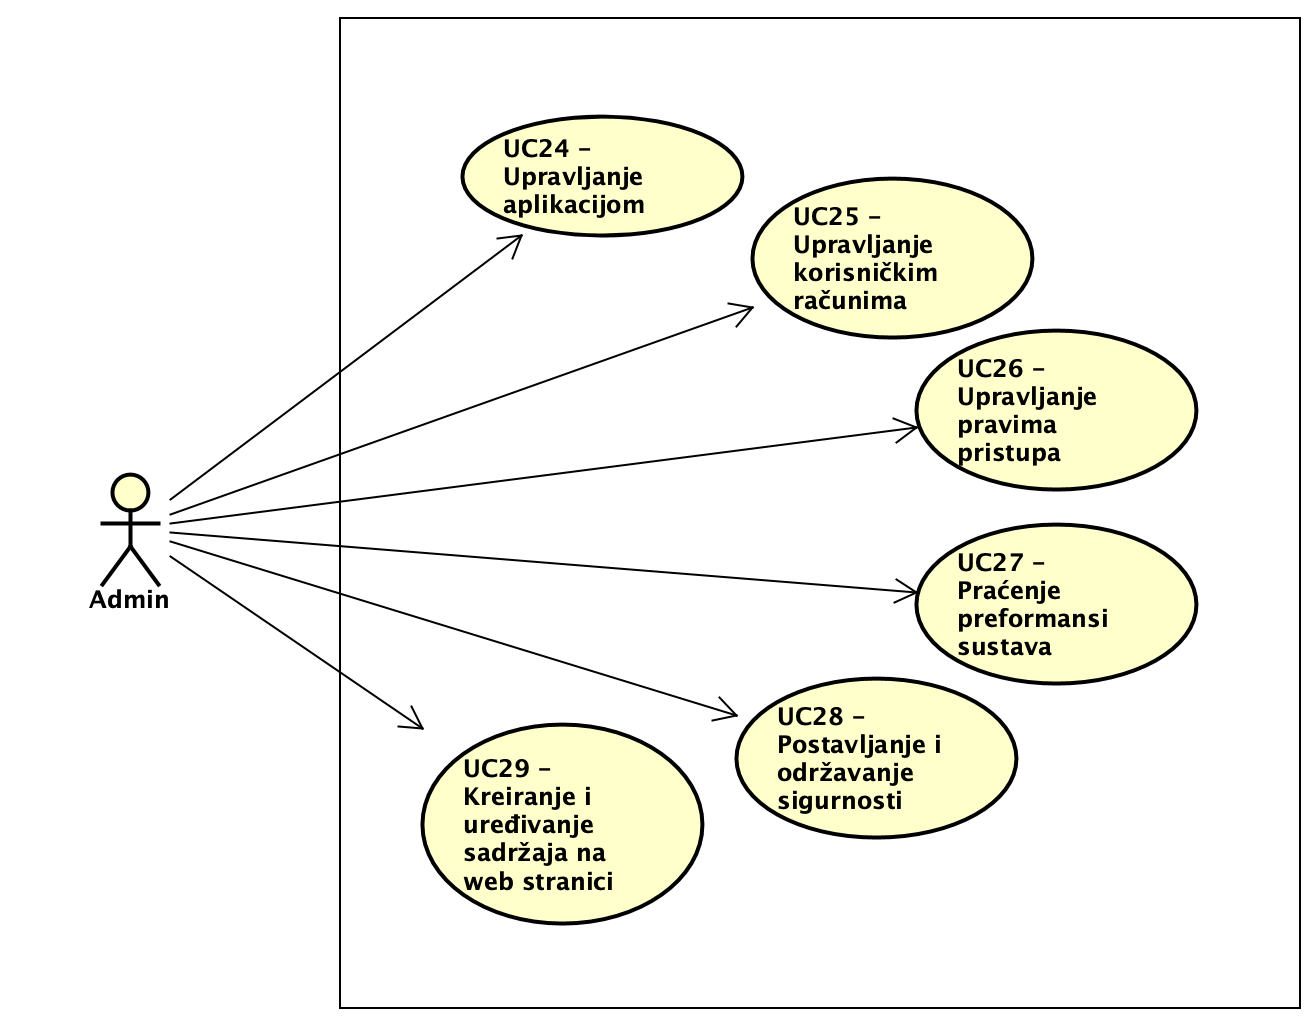
\includegraphics[scale=0.4]{slike/Dijagrami/DOU_admin.PNG} %veličina slike u odnosu na originalnu datoteku i pozicija slike
						\centering
						\caption{Dijagram uporabe obrazaca za admina}
						\label{fig:promjene}
					\end{figure}
					\begin{figure}[H]
						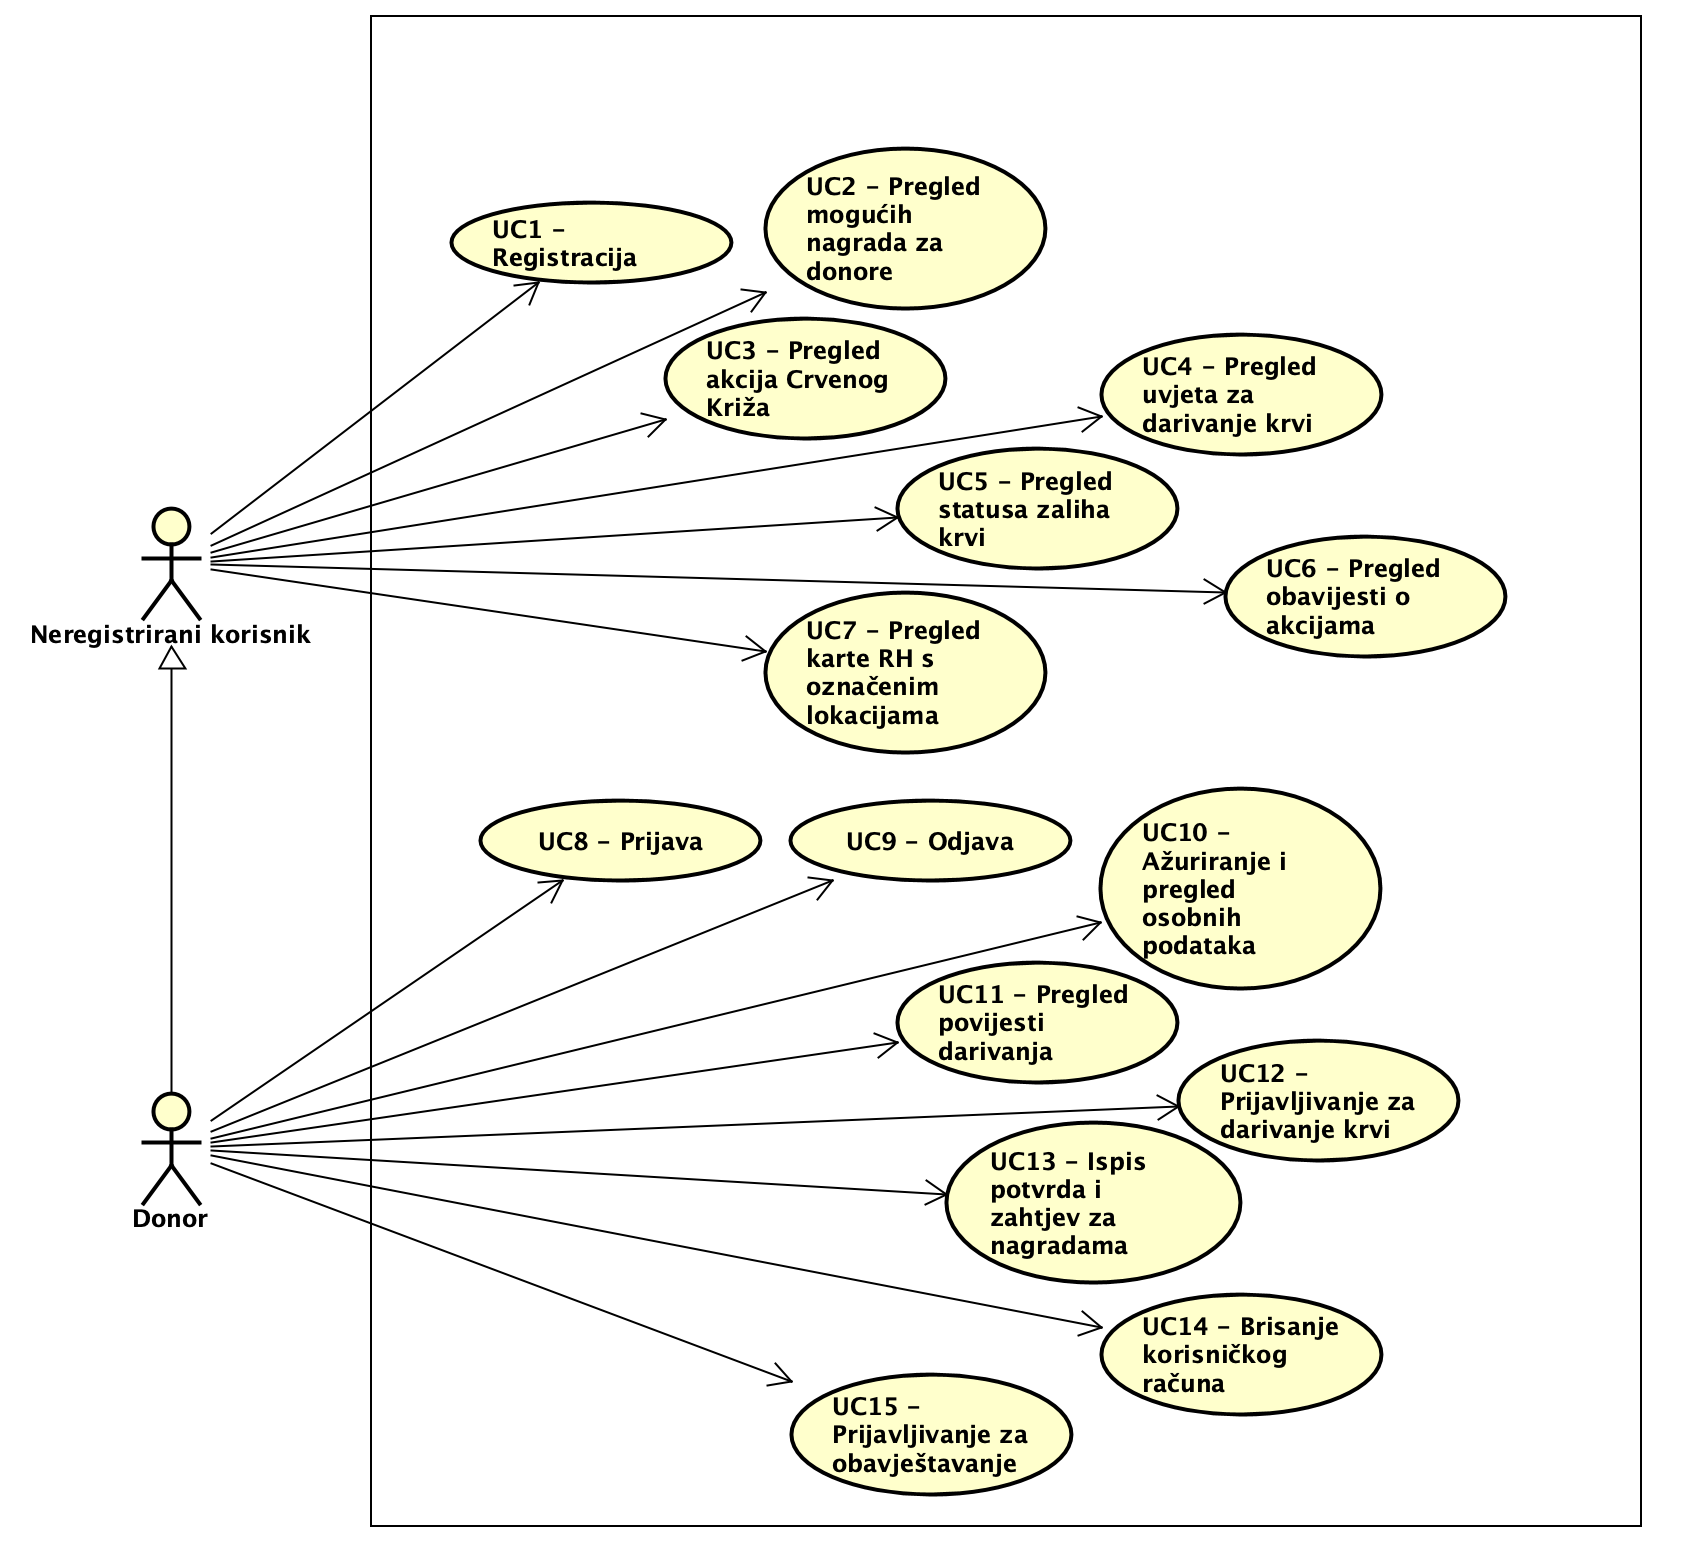
\includegraphics[scale=0.4]{slike/Dijagrami/DOU_donor.PNG} %veličina slike u odnosu na originalnu datoteku i pozicija slike
						\centering
						\caption{Dijagram uporabe obrazaca za donora}
						\label{fig:promjene}
					\end{figure}
					\begin{figure}[H]
						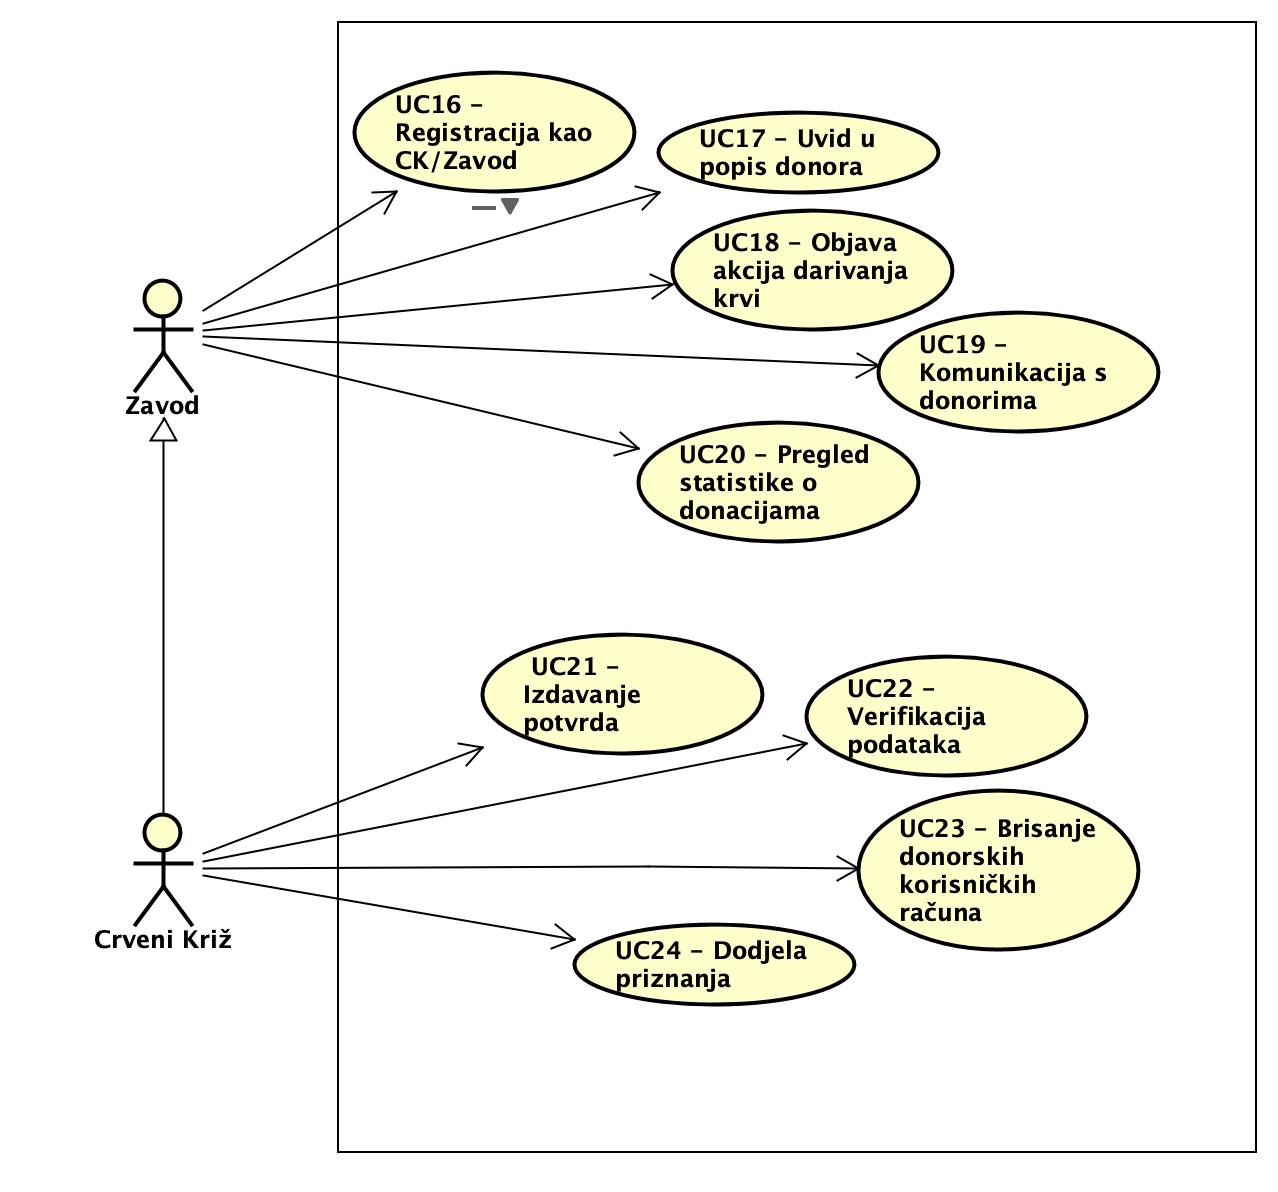
\includegraphics[scale=0.4]{slike/Dijagrami/DOU_zavod.PNG} %veličina slike u odnosu na originalnu datoteku i pozicija slike
						\centering
						\caption{Dijagram uporabe obrazaca za zavod}
						\label{fig:promjene}
					\end{figure}
				\eject		
				
			\subsection{Sekvencijski dijagrami}
				
				\textit{Nacrtati sekvencijske dijagrame koji modeliraju najvažnije dijelove sustava (max. 4 dijagrama). Ukoliko postoji nedoumica oko odabira, razjasniti s asistentom. Uz svaki dijagram napisati detaljni opis dijagrama.}
				\begin{figure}[H]
					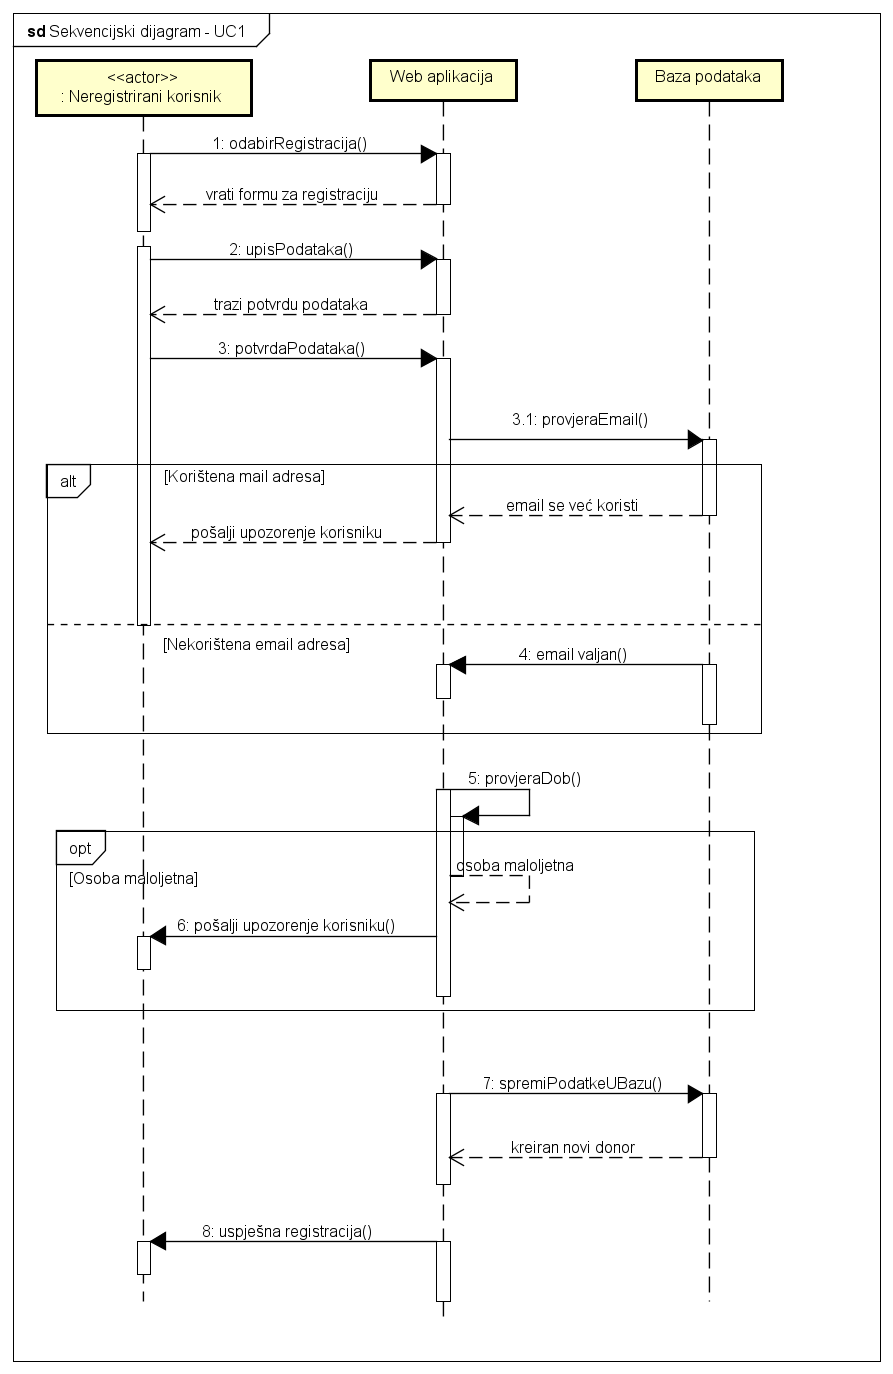
\includegraphics[scale=0.4]{slike/Dijagrami/Sekvencijski dijagram - UC1} %veličina slike u odnosu na originalnu datoteku i pozicija slike
					\centering
					\caption{Sekvencijski dijagram UC1}
					\label{fig:promjene}
				\end{figure}
				\begin{figure}[H]
					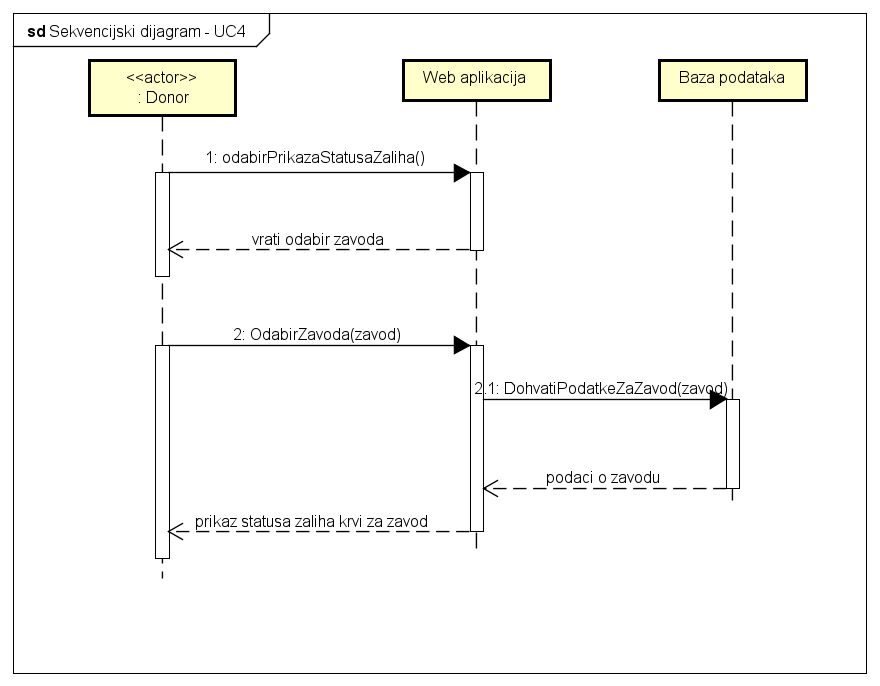
\includegraphics[scale=0.4]{slike/Dijagrami/Sekvencijski dijagram - UC4} %veličina slike u odnosu na originalnu datoteku i pozicija slike
					\centering
					\caption{Sekvencijski dijagram UC4}
					\label{fig:promjene}
				\end{figure}
				\begin{figure}[H]
					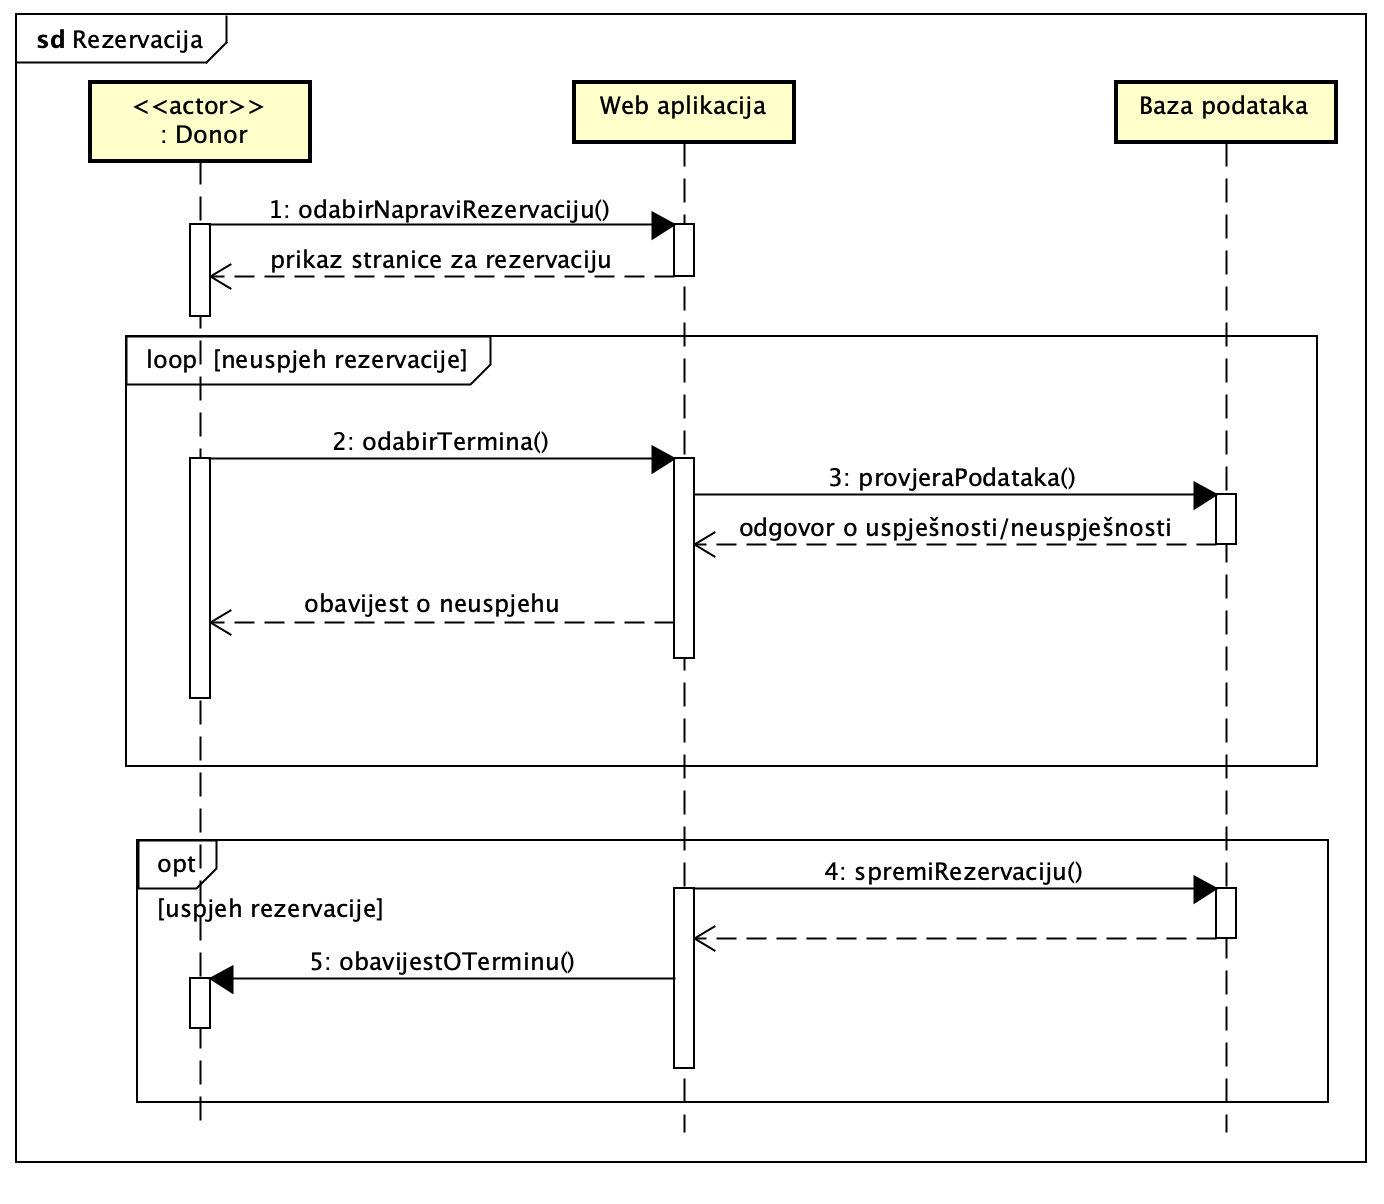
\includegraphics[scale=0.4]{slike/Dijagrami/Sekvencijski dijagram - UC11} %veličina slike u odnosu na originalnu datoteku i pozicija slike
					\centering
					\caption{Sekvencijski dijagram UC11}
					\label{fig:promjene}
				\end{figure}
				\begin{figure}[H]
					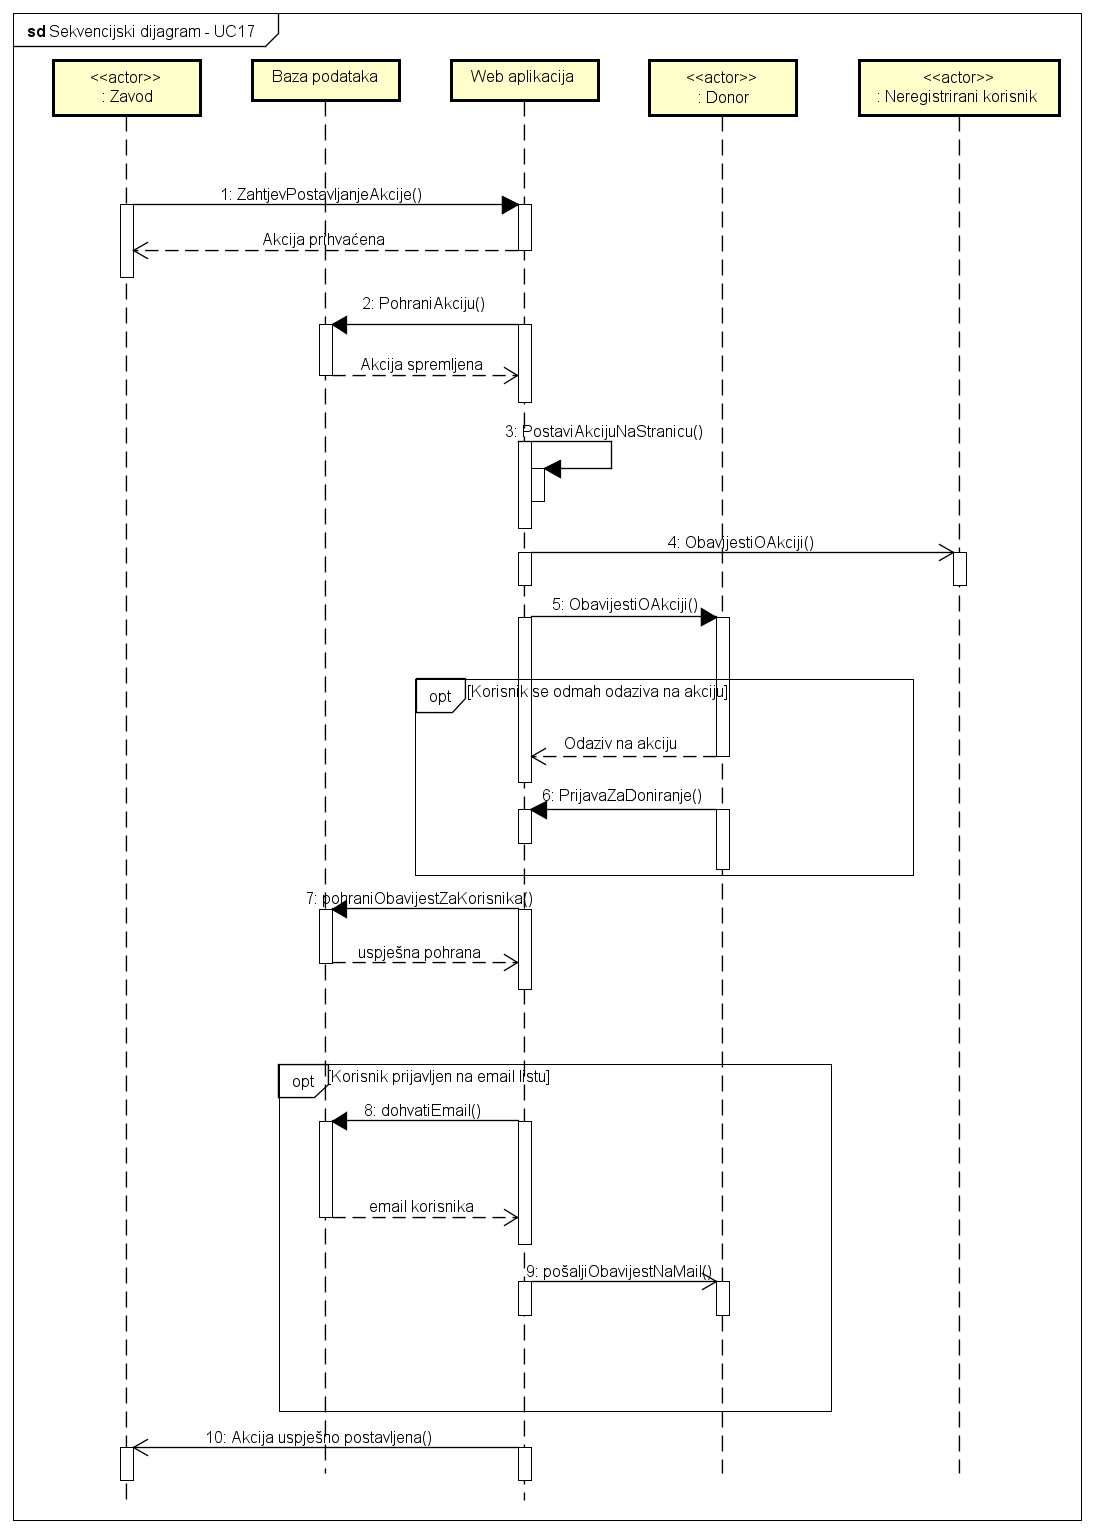
\includegraphics[scale=0.4]{slike/Dijagrami/Sekvencijski dijagram - UC17} %veličina slike u odnosu na originalnu datoteku i pozicija slike
					\centering
					\caption{Sekvencijski dijagram UC71}
					\label{fig:promjene}
				\end{figure}
				\eject
	
		\section{Ostali zahtjevi}
		
			\begin{packed_item}

				\item Sustav treba podržavati rad više korisnika u stvarnom vremenu
				\item Sustav treba biti izveden kao web aplikacija ispravno funkcionalna u svim web preglednicima
				\item	 Sustavu pristupaju registrirani korisnici pomoću korisničkog imena i pouzdane lozinke
				\item Sustav treba koristiti srednjoeuropsko strandardno vrijeme, GTM+1
				\item Sustav treba biti jednostavan i razumljiv svim korisnicima bez detaljnih uputa
				\item Sustav treba podržavati hrvatsku abecedu, uključujući dijakritičke znakove
				\item Na klijentskoj strani potrebno je implementirati korisničko sučelje koristeći React
				\item Na poslužiteljskoj strani je potrebno koristiti radni okvir Sequlize
				\item Podatke treba spremati u bazu podataka koristeći SQL?
				\item Sustav treba koristiti srednjoeuropsko strandardno vrijeme, GTM+1
				\item Sustav treba biti jednostavan i razumljiv svim korisnicima bez detaljnih uputa
				\item Sustav treba podržavati hrvatsku abecedu, uključujući dijakritičke znakove
			\end{packed_item}

			 
			 
	
	\chapter{Arhitektura i dizajn sustava}
		
		\textbf{\textit{dio 1. revizije}}\\

		\textit{ Potrebno je opisati stil arhitekture te identificirati: podsustave, preslikavanje na radnu platformu, spremišta podataka, mrežne protokole, globalni upravljački tok i sklopovsko-programske zahtjeve. Po točkama razraditi i popratiti odgovarajućim skicama:}
	\begin{itemize}
		\item 	\textit{izbor arhitekture temeljem principa oblikovanja pokazanih na predavanjima (objasniti zašto ste baš odabrali takvu arhitekturu)}
		\item 	\textit{organizaciju sustava s najviše razine apstrakcije (npr. klijent-poslužitelj, baza podataka, datotečni sustav, grafičko sučelje)}
		\item 	\textit{organizaciju aplikacije (npr. slojevi frontend i backend, MVC arhitektura) }		
	\end{itemize}

	
		

		

				
		\section{Baza podataka}
			
			\textbf{\textit{dio 1.b revizije}}\\
			
		\textit{Potrebno je opisati koju vrstu i implementaciju baze podataka ste odabrali, glavne komponente od kojih se sastoji i slično.}
		
			\subsection{Opis tablica}
			

				\textit{Svaku tablicu je potrebno opisati po zadanom predlošku. Lijevo se nalazi točno ime varijable u bazi podataka, u sredini se nalazi tip podataka, a desno se nalazi opis varijable. Svjetlozelenom bojom označite primarni ključ. Svjetlo plavom označite strani ključ}
				
				\noindent\textbf{Donors (Donatori)} tablica pohranjuje informacije o donatorima, uključujući njihovo ime, email adresu, lozinku, krvnu grupu, povezani institut za transfuziju, broj donacija te datume stvaranja i ažuriranja zapisa. Ovaj entitet je u vezi \textit{One-to-Many} s \textbf{Donations} preko \textit{id},  {Many-to-One} s \textbf{BloodBanks} preko \textit{transfusionInstitute}, \textit{One-to-Many} s \textbf{Certificates} preko \textit{id} i \textit{One-to-Many} s \textbf{ActionRegistrations} preko \textit{id}.
				\begin{table}[H]
				    \renewcommand{\arraystretch}{2}
				    \centering
				     \begin{tabularx}{1\textwidth}{|c|c|X|}
				    \hline
				    \textbf{Naziv Stupca} & \textbf{Vrsta podatka} & \textbf{Opis} \\
				    \hline
				    \cellcolor{LightGreen} id & INTEGER & Automatski povećavajući broj\\
				    \hline
				    name & STRING & Ime donatora \\
				    \hline 
				     email & STRING & Email adresa donatora \\ 
				    \hline
				    password & STRING & Lozinka donatora \\
				    \hline
				    bloodType & STRING & Krvna grupa donatora \\
				    \hline
				    \cellcolor{LightBlue} transfusionInstitute & STRING & Institut za transfuziju zadužen za donatora\\
				    \hline
				    numberOfDonations & INTEGER & Broj donacija donatora \\
				    \hline
				    createdAt & TIMESTAMP & Datum i vrijeme stvaranja zapisa \\
				    \hline
				    updatedAt & TIMESTAMP & Datum i vrijeme posljednjeg ažuriranja zapisa \\
				    \hline
				    \end{tabularx}
				    \caption{Donors}
				    \label{tab:my_label}
				\end{table}
				\clearpage % Start a new page
				
				\noindent\textbf{Donations (Donacije)} tablica sadrži informacije o donacijama, uključujući datum donacije, adresu, upozorenje te podatke o povezanom donatoru. Također, sadrži datume stvaranja i ažuriranja zapisa. Ovaj entitet je u vezi \textit{Many-to-One} s \textbf{Donors} preko \textit{donorId}.
				\begin{table}[H]
				    \renewcommand{\arraystretch}{2}
				    \centering
				     \begin{tabularx}{1\textwidth}{|c|c|X|}
				    \hline
				    \textbf{Naziv Stupca} & \textbf{Vrsta podatka} & \textbf{Opis} \\
				    \hline
				    \cellcolor{LightGreen}id & INTEGER & Automatski povećavajući broj\\
				    \hline
				    date & DATE & Datum donacije \\
				    \hline
				    address & STRING & Adresa donacije \\
				    \hline
				    warning & STRING & Upozorenje ako krv nije bila potpuno zdrava \\
				    \hline
				    createdAt & TIMESTAMP & Datum i vrijeme stvaranja zapisa \\
				    \hline
				    updatedAt & TIMESTAMP & Datum i vrijeme posljednjeg ažuriranja zapisa \\
				    \hline
				    \cellcolor{LightBlue} donorId & INTEGER & ID donatora  \\
				    \hline
				    \end{tabularx}
				    \caption{Donations}
				    \label{tab:my_label}
				\end{table}
				\clearpage % Start a new page
				
				\noindent\textbf{Certificates (Certifikati)} tablica pohranjuje informacije o certifikatima koje donatori mogu postići. Uključuje naziv certifikata, njegove pogodnosti, broj donacija potreban za certifikat te datume stvaranja i ažuriranja zapisa. Također, sadrži podatke o povezanom donatoru. Ovaj entitet je u vezi \textit{Many-to-One} s \textbf{Donors} preko \textit{donorId}.
				\begin{table}[H]
				    \renewcommand{\arraystretch}{2}
				    \centering
				     \begin{tabularx}{1\textwidth}{|c|c|X|}
				    \hline
				    \textbf{Naziv Stupca} & \textbf{Vrsta podatka} & \textbf{Opis} \\
				    \hline
				    \cellcolor{LightGreen} id & INTEGER & Automatski povećavajući broj\\
				    \hline
				    name & STRING & Naziv certifikata \\
				    \hline
				    benefits & STRING & Pogodnosti certifikata \\
				    \hline
				    numberOfDonations & INTEGER & Broj donacija potreban za certifikat \\
				    \hline
				    createdAt & TIMESTAMP & Datum i vrijeme stvaranja zapisa \\
				    \hline
				    updatedAt & TIMESTAMP & Datum i vrijeme posljednjeg ažuriranja zapisa \\
				    \hline
				    \cellcolor{LightBlue} donorId & INTEGER & ID donatora \\
				    \hline
				    \end{tabularx}
				    \caption{Certificates}
				    \label{tab:my_label}
				\end{table}
				\clearpage % Start a new page
				
				\noindent\textbf{BloodBanks (Zavodi za Transfuziju)} tablica pohranjuje informacije o zavodima za transfuziju krvi, uključujući naziv zavoda za transfuziju, adresu, broj donatora povezanih s zavodom za transfuziju te datume stvaranja i ažuriranja zapisa. Ovaj entitet je u vezi \textit{One-to-Many} s \textbf{Donors} preko \textit{id}.
				\begin{table}[H]
				    \renewcommand{\arraystretch}{2}
				    \centering
				     \begin{tabularx}{1\textwidth}{|c|c|X|}
				    \hline
				    \textbf{Naziv Stupca} & \textbf{Vrsta podatka} & \textbf{Opis} \\
				    \hline
				    \cellcolor{LightGreen} id & INTEGER & Automatski povećavajući broj\\
				    \hline
				    name & STRING & Naziv zavoda \\
				    \hline
				    email & STRING & Email adresa zavoda \\
				    \hline
				    password & STRING & Lozinka zavoda \\
				    \hline
				    address & STRING & Adresa zavoda \\
				    \hline
				    numberOfDonors & INTEGER & Broj donatora povezan sa zavodom \\
				    \hline
				    createdAt & TIMESTAMP & Datum i vrijeme stvaranja zapisa \\
				    \hline
				    updatedAt & TIMESTAMP & Datum i vrijeme posljednjeg ažuriranja zapisa \\
				    \hline
				    \end{tabularx}
				    \caption{BloodBanks}
				    \label{tab:my_label}
				\end{table}
				\clearpage % Start a new page
				
				\noindent\textbf{Actions (Akcije)} tablica pohranjuje informacije o akcijama koje uključuju adresu, datum, minimalni broj donatora potreban za akciju te datume stvaranja i ažuriranja zapisa. Također, sadrži podatak o povezanom zavodu. Ovaj entitet je u vezi \textit{Many-to-One} s \textbf{BloodBanks} preko \textit{bloodBankId}.
				\begin{table}[H]
				    \renewcommand{\arraystretch}{2}
				    \centering
				     \begin{tabularx}{1\textwidth}{|c|c|X|}
				    \hline
				    \textbf{Naziv Stupca} & \textbf{Vrsta podatka} & \textbf{Opis} \\
				    \hline
				    \cellcolor{LightGreen}id & INTEGER & Automatski povećavajući broj\\
				    \hline
				    address & STRING & Adresa akcije \\
				    \hline
				    date & DATE & Datum akcije \\
				    \hline
				    minNumberOfDonors & INTEGER & Minimalni broj donatora potreban za akciju \\
				    \hline
				    createdAt & TIMESTAMP & Datum i vrijeme stvaranja zapisa \\
				    \hline
				    updatedAt & TIMESTAMP & Datum i vrijeme posljednjeg ažuriranja zapisa \\
				    \hline
				    \cellcolor{LightBlue} bloodBankId & INTEGER & ID zavoda \\
				    \hline
				    \end{tabularx}
				    \caption{Actions}
				    \label{tab:my_label}
				\end{table}
				\clearpage % Start a new page
				
				\noindent\textbf{ActionRegistrations (Registracije za Akcije)} tablica sadrži informacije o registracijama za akcije. Uključuje ID akcije, ID donatora te datume stvaranja i ažuriranja zapisa. Ovaj entitet je u vezi \textit{Many-to-One} s \textbf{Actions} preko \textit{actionId} i \textit{Many-to-One} s \textbf{Donors} preko \textit{donorId}.
				\begin{table}[H]
				    \renewcommand{\arraystretch}{2}
				    \centering
				     \begin{tabularx}{1\textwidth}{|c|c|X|}
				    \hline
				    \textbf{Naziv Stupca} & \textbf{Vrsta podatka} & \textbf{Opis} \\
				    \hline
				    \cellcolor{LightGreen} id & INTEGER & Automatski povećavajući broj\\
				    \hline
				    \cellcolor{LightBlue} actionId & INTEGER & ID akcije  \\
				    \hline
				    \cellcolor{LightGreen}donorId & INTEGER & ID donatora \\
				    \hline
				    createdAt & TIMESTAMP & Datum i vrijeme stvaranja zapisa \\
				    \hline
				    updatedAt & TIMESTAMP & Datum i vrijeme posljednjeg ažuriranja zapisa \\
				    \hline
				    \end{tabularx}
				    \caption{ActionRegistrations}
				    \label{tab:my_label}
				\end{table}
				\clearpage % Start a new page

				
				\begin{longtblr}[
					label=none,
					entry=none
					]{
						width = \textwidth,
						colspec={|X[6,l]|X[6, l]|X[20, l]|}, 
						rowhead = 1,
					} %definicija širine tablice, širine stupaca, poravnanje i broja redaka naslova tablice
					\hline \SetCell[c=3]{c}{\textbf{korisnik - ime tablice}}	 \\ \hline[3pt]
					\SetCell{LightGreen}IDKorisnik & INT	&  	Lorem ipsum dolor sit amet, consectetur adipiscing elit, sed do eiusmod  	\\ \hline
					korisnickoIme	& VARCHAR &   	\\ \hline 
					email & VARCHAR &   \\ \hline 
					ime & VARCHAR	&  		\\ \hline 
					\SetCell{LightBlue} primjer	& VARCHAR &   	\\ \hline 
				\end{longtblr}
				
				
				
				
			
			\subsection{Dijagram baze podataka}
				\textit{ U ovom potpoglavlju potrebno je umetnuti dijagram baze podataka. Primarni i strani ključevi moraju biti označeni, a tablice povezane. Bazu podataka je potrebno normalizirati. Podsjetite se kolegija "Baze podataka".}
			
			\eject
			
			
		\section{Dijagram razreda}
		
			\textit{Potrebno je priložiti dijagram razreda s pripadajućim opisom. Zbog preglednosti je moguće dijagram razlomiti na više njih, ali moraju biti grupirani prema sličnim razinama apstrakcije i srodnim funkcionalnostima.}\\
			
			\textbf{\textit{dio 1. revizije}}\\
			
			\textit{Prilikom prve predaje projekta, potrebno je priložiti potpuno razrađen dijagram razreda vezan uz \textbf{generičku funkcionalnost} sustava. Ostale funkcionalnosti trebaju biti idejno razrađene u dijagramu sa sljedećim komponentama: nazivi razreda, nazivi metoda i vrste pristupa metodama (npr. javni, zaštićeni), nazivi atributa razreda, veze i odnosi između razreda.}\\
			
			\textbf{\textit{dio 2. revizije}}\\			
			
			\textit{Prilikom druge predaje projekta dijagram razreda i opisi moraju odgovarati stvarnom stanju implementacije}
			
			
			
			\eject
		
		\section{Dijagram stanja}
			
			
			\textbf{\textit{dio 2. revizije}}\\
			
			\textit{Potrebno je priložiti dijagram stanja i opisati ga. Dovoljan je jedan dijagram stanja koji prikazuje \textbf{značajan dio funkcionalnosti} sustava. Na primjer, stanja korisničkog sučelja i tijek korištenja neke ključne funkcionalnosti jesu značajan dio sustava, a registracija i prijava nisu. }
			
			
			\eject 
		
		\section{Dijagram aktivnosti}
			
			\textbf{\textit{dio 2. revizije}}\\
			
			 \textit{Potrebno je priložiti dijagram aktivnosti s pripadajućim opisom. Dijagram aktivnosti treba prikazivati značajan dio sustava.}
			
			\eject
		\section{Dijagram komponenti}
		
			\textbf{\textit{dio 2. revizije}}\\
		
			 \textit{Potrebno je priložiti dijagram komponenti s pripadajućim opisom. Dijagram komponenti treba prikazivati strukturu cijele aplikacije.}
	\chapter{Implementacija i korisničko sučelje}
		
		
		\section{Korištene tehnologije i alati}
		
			\textbf{\textit{dio 2. revizije}}
			
			 \textit{Detaljno navesti sve tehnologije i alate koji su primijenjeni pri izradi dokumentacije i aplikacije. Ukratko ih opisati, te navesti njihovo značenje i mjesto primjene. Za svaki navedeni alat i tehnologiju je potrebno \textbf{navesti internet poveznicu} gdje se mogu preuzeti ili više saznati o njima}.
			
			
			\eject 
		
	
		\section{Ispitivanje programskog rješenja}
			
			\textbf{\textit{dio 2. revizije}}\\
			
			 \textit{U ovom poglavlju je potrebno opisati provedbu ispitivanja implementiranih funkcionalnosti na razini komponenti i na razini cijelog sustava s prikazom odabranih ispitnih slučajeva. Studenti trebaju ispitati temeljnu funkcionalnost i rubne uvjete.}
	
			
			\subsection{Ispitivanje komponenti}
			\textit{Potrebno je provesti ispitivanje jedinica (engl. unit testing) nad razredima koji implementiraju temeljne funkcionalnosti. Razraditi \textbf{minimalno 6 ispitnih slučajeva} u kojima će se ispitati redovni slučajevi, rubni uvjeti te izazivanje pogreške (engl. exception throwing). Poželjno je stvoriti i ispitni slučaj koji koristi funkcionalnosti koje nisu implementirane. Potrebno je priložiti izvorni kôd svih ispitnih slučajeva te prikaz rezultata izvođenja ispita u razvojnom okruženju (prolaz/pad ispita). }
			
			
			
			\subsection{Ispitivanje sustava}
			
			 \textit{Potrebno je provesti i opisati ispitivanje sustava koristeći radni okvir Selenium\footnote{\url{https://www.seleniumhq.org/}}. Razraditi \textbf{minimalno 4 ispitna slučaja} u kojima će se ispitati redovni slučajevi, rubni uvjeti te poziv funkcionalnosti koja nije implementirana/izaziva pogrešku kako bi se vidjelo na koji način sustav reagira kada nešto nije u potpunosti ostvareno. Ispitni slučaj se treba sastojati od ulaza (npr. korisničko ime i lozinka), očekivanog izlaza ili rezultata, koraka ispitivanja i dobivenog izlaza ili rezultata.\\ }
			 
			 \textit{Izradu ispitnih slučajeva pomoću radnog okvira Selenium moguće je provesti pomoću jednog od sljedeća dva alata:}
			 \begin{itemize}
			 	\item \textit{dodatak za preglednik \textbf{Selenium IDE} - snimanje korisnikovih akcija radi automatskog ponavljanja ispita	}
			 	\item \textit{\textbf{Selenium WebDriver} - podrška za pisanje ispita u jezicima Java, C\#, PHP koristeći posebno programsko sučelje.}
			 \end{itemize}
		 	\textit{Detalji o korištenju alata Selenium bit će prikazani na posebnom predavanju tijekom semestra.}
			
			\eject 
		
		
		\section{Dijagram razmještaja}
			
			\textbf{\textit{dio 2. revizije}}
			
			 \textit{Potrebno je umetnuti \textbf{specifikacijski} dijagram razmještaja i opisati ga. Moguće je umjesto specifikacijskog dijagrama razmještaja umetnuti dijagram razmještaja instanci, pod uvjetom da taj dijagram bolje opisuje neki važniji dio sustava.}
			
			\eject 
		
		\section{Upute za puštanje u pogon}
		
			\textbf{\textit{dio 2. revizije}}\\
		
			 \textit{U ovom poglavlju potrebno je dati upute za puštanje u pogon (engl. deployment) ostvarene aplikacije. Na primjer, za web aplikacije, opisati postupak kojim se od izvornog kôda dolazi do potpuno postavljene baze podataka i poslužitelja koji odgovara na upite korisnika. Za mobilnu aplikaciju, postupak kojim se aplikacija izgradi, te postavi na neku od trgovina. Za stolnu (engl. desktop) aplikaciju, postupak kojim se aplikacija instalira na računalo. Ukoliko mobilne i stolne aplikacije komuniciraju s poslužiteljem i/ili bazom podataka, opisati i postupak njihovog postavljanja. Pri izradi uputa preporučuje se \textbf{naglasiti korake instalacije uporabom natuknica} te koristiti što je više moguće \textbf{slike ekrana} (engl. screenshots) kako bi upute bile jasne i jednostavne za slijediti.}
			
			
			 \textit{Dovršenu aplikaciju potrebno je pokrenuti na javno dostupnom poslužitelju. Studentima se preporuča korištenje neke od sljedećih besplatnih usluga: \href{https://aws.amazon.com/}{Amazon AWS}, \href{https://azure.microsoft.com/en-us/}{Microsoft Azure} ili \href{https://www.heroku.com/}{Heroku}. Mobilne aplikacije trebaju biti objavljene na F-Droid, Google Play ili Amazon App trgovini.}
			
			
			\eject 
	\chapter{Zaključak i budući rad}
		
		\textbf{\textit{dio 2. revizije}}\\
		
		 \textit{U ovom poglavlju potrebno je napisati osvrt na vrijeme izrade projektnog zadatka, koji su tehnički izazovi prepoznati, jesu li riješeni ili kako bi mogli biti riješeni, koja su znanja stečena pri izradi projekta, koja bi znanja bila posebno potrebna za brže i kvalitetnije ostvarenje projekta i koje bi bile perspektive za nastavak rada u projektnoj grupi.}
		
		 \textit{Potrebno je točno popisati funkcionalnosti koje nisu implementirane u ostvarenoj aplikaciji.}
		
		\eject 
	\chapter*{Popis literature}
		\addcontentsline{toc}{chapter}{Popis literature}
	 	
 		\textbf{\textit{Kontinuirano osvježavanje}}
	
		\textit{Popisati sve reference i literaturu koja je pomogla pri ostvarivanju projekta.}
		
		
		\begin{enumerate}
			
			
			\item  Programsko inženjerstvo, FER ZEMRIS, \url{http://www.fer.hr/predmet/proinz}
			
			\item  I. Sommerville, "Software engineering", 8th ed, Addison Wesley, 2007.
			
			\item  T.C.Lethbridge, R.Langaniere, "Object-Oriented Software Engineering", 2nd ed. McGraw-Hill, 2005.
			
			\item  I. Marsic, Software engineering book``, Department of Electrical and Computer Engineering, Rutgers University, \url{http://www.ece.rutgers.edu/~marsic/books/SE}
			
			\item  The Unified Modeling Language, \url{https://www.uml-diagrams.org/}
			
			\item  Astah Community, \url{http://astah.net/editions/uml-new}
		\end{enumerate}
		
		 
	
	
	\begingroup
	\renewcommand*\listfigurename{Indeks slika i dijagrama}
	%\renewcommand*\listtablename{Indeks tablica}
	%\let\clearpage\relax
	\listoffigures
	%\vspace{10mm}
	%\listoftables
	\endgroup
	\addcontentsline{toc}{chapter}{Indeks slika i dijagrama}


	
	\eject 
		
	\chapter*{Dodatak: Prikaz aktivnosti grupe}
		\addcontentsline{toc}{chapter}{Dodatak: Prikaz aktivnosti grupe}
		
		\section*{Dnevnik sastajanja}
		
		\textbf{\textit{Kontinuirano osvježavanje}}\\
		
		 \textit{U ovom dijelu potrebno je redovito osvježavati dnevnik sastajanja prema predlošku.}
		
		\begin{packed_enum}
			\item  sastanak
			
			\item[] \begin{packed_item}
				\item Datum: u ovom formatu: \today
				\item Prisustvovali: I.Prezime, I.Prezime
				\item Teme sastanka:
				\begin{packed_item}
					\item  opis prve teme
					\item  opis druge teme
				\end{packed_item}
			\end{packed_item}
			
			\item  sastanak
			\item[] \begin{packed_item}
				\item Datum: u ovom formatu: \today
				\item Prisustvovali: I.Prezime, I.Prezime
				\item Teme sastanka:
				\begin{packed_item}
					\item  opis prve teme
					\item  opis druge teme
				\end{packed_item}
			\end{packed_item}
			
			%
			
		\end{packed_enum}
		
		\eject
		\section*{Tablica aktivnosti}
		
			\textbf{\textit{Kontinuirano osvježavanje}}\\
			
			 \textit{Napomena: Doprinose u aktivnostima treba navesti u satima po članovima grupe po aktivnosti.}

			\begin{longtblr}[
					label=none,
				]{
					vlines,hlines,
					width = \textwidth,
					colspec={X[7, l]X[1, c]X[1, c]X[1, c]X[1, c]X[1, c]X[1, c]X[1, c]}, 
					vline{1} = {1}{text=\clap{}},
					hline{1} = {1}{text=\clap{}},
					rowhead = 1,
				} 
			
				\SetCell[c=1]{c}{} & \SetCell[c=1]{c}{\rotatebox{90}{\textbf{Ime Prezime voditelja}}} & \SetCell[c=1]{c}{\rotatebox{90}{\textbf{Ime Prezime }}} &	\SetCell[c=1]{c}{\rotatebox{90}{\textbf{Ime Prezime }}} & \SetCell[c=1]{c}{\rotatebox{90}{\textbf{Ime Prezime }}} &	\SetCell[c=1]{c}{\rotatebox{90}{\textbf{Ime Prezime }}} & \SetCell[c=1]{c}{\rotatebox{90}{\textbf{Ime Prezime }}} &	\SetCell[c=1]{c}{\rotatebox{90}{\textbf{Ime Prezime }}} \\  
				Upravljanje projektom 		&  &  &  &  &  &  & \\ 
				Opis projektnog zadatka 	&  &  &  &  &  &  & \\ 
				
				Funkcionalni zahtjevi       &  &  &  &  &  &  &  \\ 
				Opis pojedinih obrazaca 	&  &  &  &  &  &  &  \\ 
				Dijagram obrazaca 			&  &  &  &  &  &  &  \\ 
				Sekvencijski dijagrami 		&  &  &  &  &  &  &  \\ 
				Opis ostalih zahtjeva 		&  &  &  &  &  &  &  \\ 

				Arhitektura i dizajn sustava	 &  &  &  &  &  &  &  \\ 
				Baza podataka				&  &  &  &  &  &  &   \\ 
				Dijagram razreda 			&  &  &  &  &  &  &   \\ 
				Dijagram stanja				&  &  &  &  &  &  &  \\ 
				Dijagram aktivnosti 		&  &  &  &  &  &  &  \\ 
				Dijagram komponenti			&  &  &  &  &  &  &  \\ 
				Korištene tehnologije i alati 		&  &  &  &  &  &  &  \\ 
				Ispitivanje programskog rješenja 	&  &  &  &  &  &  &  \\ 
				Dijagram razmještaja			&  &  &  &  &  &  &  \\ 
				Upute za puštanje u pogon 		&  &  &  &  &  &  &  \\  
				Dnevnik sastajanja 			&  &  &  &  &  &  &  \\ 
				Zaključak i budući rad 		&  &  &  &  &  &  &  \\  
				Popis literature 			&  &  &  &  &  &  &  \\  
				&  &  &  &  &  &  &  \\ \hline 
				\textit{Dodatne stavke kako ste podijelili izradu aplikacije} 			&  &  &  &  &  &  &  \\ 
				\textit{npr. izrada početne stranice} 				&  &  &  &  &  &  &  \\  
				\textit{izrada baze podataka} 		 			&  &  &  &  &  &  & \\  
				\textit{spajanje s bazom podataka} 							&  &  &  &  &  &  &  \\ 
				\textit{back end} 							&  &  &  &  &  &  &  \\  
				 							&  &  &  &  &  &  &\\ 
			\end{longtblr}
					
					
		\eject
		\section*{Dijagrami pregleda promjena}
		
		\textbf{\textit{dio 2. revizije}}\\
		
		\textit{Prenijeti dijagram pregleda promjena nad datotekama projekta. Potrebno je na kraju projekta generirane grafove s gitlaba prenijeti u ovo poglavlje dokumentacije. Dijagrami za vlastiti projekt se mogu preuzeti s gitlab.com stranice, u izborniku Repository, pritiskom na stavku Contributors.}
		
	


\end{document} %naredbe i tekst nakon ove naredbe ne ulaze u izgrađen dokument 


